\documentclass[12pt]{report}

\usepackage{pdfpages}

\usepackage{graphicx}
\graphicspath{ {figures/} }
\graphicspath{{images/}}
\usepackage[margin=1 in, includefoot]{Geometry}
\usepackage{hyperref}
\hypersetup{colorlinks=true,linkcolor=blue,urlcolor=cyan,}
%pdfpagemode=fullScreen}
\usepackage[english]{babel}
\usepackage[utf8]{inputenc}
\usepackage{fancyhdr}
\pagestyle{fancy}
\fancyhf{}
\renewcommand{\headrulewidth}{0pt}
\renewcommand{\footrulewidth}{1pt}
\usepackage{ragged2e}
\usepackage{times}
\usepackage{array}
\renewcommand\thesection{\arabic{section}}
\usepackage {hyperref}
\usepackage{graphicx,wrapfig,lipsum}
\usepackage{array}
\usepackage{multirow}

\DeclareUnicodeCharacter{0394}{\ensuremath{\Delta}}

%header and footer
\cfoot{\fontsize{10}{12} \selectfont DYPIT, Department of Computer Engineering 2022-2023 }
%\chead{Cloud Cryptography: User End Encryption}




\begin{document}

%Start of Title page
\centering \large \textbf  {A PROJECT REPORT ON}\\
\vspace{0.75 cm}
\Large \textbf{"PC Game Development using Unity”}\\
\vspace{0.5 cm}
%\normalsize {on}\\
%\vspace{0.1 cm}
\normalsize{SUBMITTED TO THE SAVITRIBAI PHULE PUNE UNIVERSITY, PUNE}\\
\normalsize{IN THE PARTIAL FULFILLMENT OF THE REQUIREMENTS}\\
\normalsize{  FOR THE AWARD OF THE DEGREE}\\
\vspace{0.75 cm}
\normalsize {OF}\\
\vspace{0.75 cm}

\Large\textbf{BACHELOR OF COMPUTER ENGINEERING}\\
\vspace{0.8 cm}
\large{SUBMITTED BY}\\
\vspace{0.3 cm}

\large \textbf  {Ankur Patil (BCOB10)}

\large \textbf  {Lalu Nair (BCOB05) }

\large \textbf {Viren Patil (BCOB14)}

\large \textbf {Sharan Thakur (BCOB09)}
%\vspace{0.3 cm}

\begin{figure}[h]
\centering

\includegraphics[scale=0.25]{Logo.png }
\end{figure}

\centering \Large \textbf  {DEPARTMENT OF COMPUTER ENGINEERING}\\
\vspace{0.4cm}

\large \textbf  {DR. D. Y. PATIL INSTITUTE OF TECHNOLOGY}\\
\normalsize {PIMPRI, PUNE 411018}\\
\vspace{0.2 cm}
\large \textbf{SAVITRIBAI PHULE PUNE UNIVERSITY}\\


\large \textbf  {2022-2023}\\
\vspace{0.25 cm}
\thispagestyle{empty}
\clearpage
% End of Title page

% start of Certificate

%\begin{wrapfigure}{l}{5.5cm}
\begin{figure}[h]
\centering

\includegraphics[width=6cm]{Logo.png}
%\end{wrapfigure} 
\end{figure}

\vspace{0.3 cm}
\centering{\large \textbf{CERTIFICATE}\\}

\vspace{0.4 cm}

\normalsize{This is to certify that the Project Entitled}\\
\vspace{0.3cm}
\large\textbf{PC Game Development using Unity}\\
\vspace{0.3 cm}
\normalsize{Submitted by}\\
\vspace{0.3 cm}

\normalsize  {Ankur Patil (BCOB10)}

\normalsize  {Lalu Nair (BCOB05)}

\normalsize  {Viren Patil (BCOB14)}

\normalsize  {Sharan Thakur (BCOB09)}

\justifying
\setlength{\parindent}{4em}
\setlength{\parskip}{1em}
\renewcommand{\baselinestretch}{1.5}
\normalsize
are bonafide students of Dr. D. Y. Patil Institute of Technology and the work has been carried 
out by them under the supervision of Mr. Sharad Adsure (Asst. Professor) and Mrs. 
Deepika Jaiswal (Asst. Professor), it is approved for the partial fulfillment of the 
requirement of Savitribai Phule Pune University, for the award of the degree of Bachelor of Computer
Engineering.
\vspace{0.05 cm}
\linebreak

\setlength{\parindent}{-1.05em}
\setlength{\parskip}{-1.05em}

\includegraphics[scale=0.85]{firstPage-1.png}
% \setlength{\parindent}{0 em}
%  \textbf{Mr. Sharad Adsure} 
%  \hspace{5cm} 
%  \textbf{ Dr.Vinod Kimbahune  } 
%  \hspace{5.5cm}         
% \centering
% (Internal Guide)
%  \hspace{5 cm} 
%  (Head of the Department) 
%  \hspace{1 cm}    \\

% \vspace{0.4 cm}
% \setlength{\parindent}{0 em}
% \textbf{  External Examiner}   \hspace{5cm}
%  \textbf{Mrs.Sunita Patil}
% \hspace{5cm}  (Project Coordinator)  \hspace{2 cm}    \\

% \centering
% \textbf{Dr. Lalit Kumar Wadhwa}\\
%  Principal,\\
%  Dr. D. Y. Patil Institute of Technology,\\
%  Pimpri, Pune – 411018
\begin{flushleft}
Date:
\end{flushleft}

\thispagestyle{empty}
\clearpage
% End of Cerficate


% Office Certificates
\begin{figure}[h]
\centering

\includegraphics[scale=0.6]{Allocation.png}
\caption{Sponsorship Allocation Letter}
\label{Sponsorship Letter}
\end{figure}
\thispagestyle{empty}
\clearpage

\begin{figure}[h]
\centering
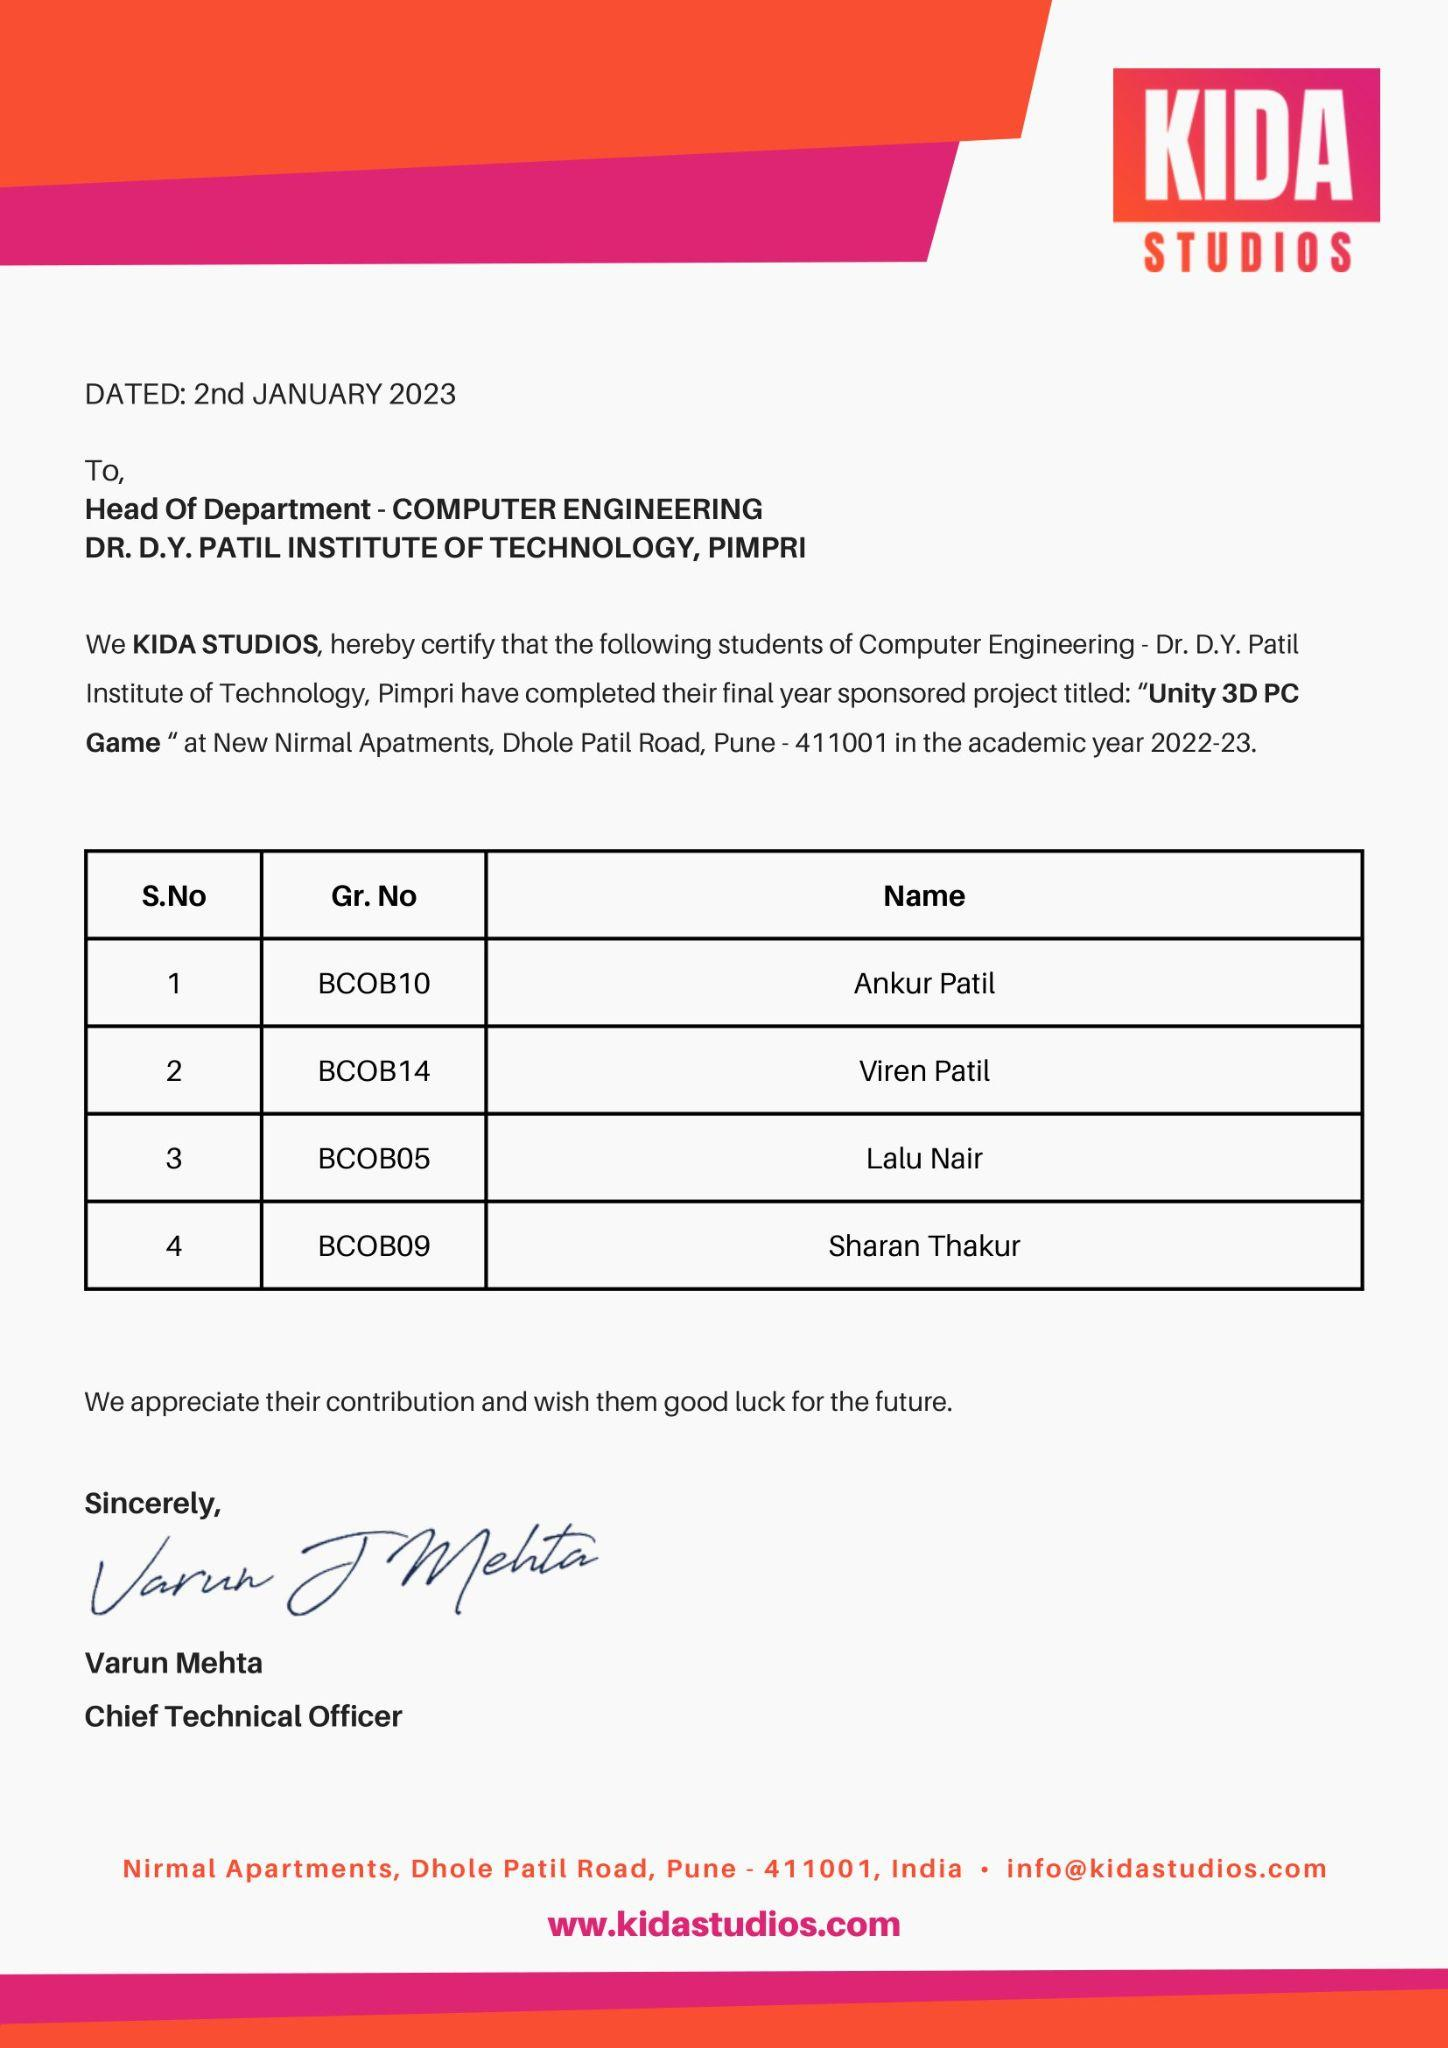
\includegraphics[scale=0.25]{image3.png}
\caption{Internship Completion Letter}
\label{Sponsorship Letter}
\end{figure}
\thispagestyle{empty}
\clearpage

% start of ACKNOWLWDGEMENT

\vspace{4 cm}
\centering{\LARGE \textbf \underline{ACKNOWLEDGEMENT}\\}
\vspace{1 cm}
\justifying
\vspace{1 cm}
\justifying
\setlength{\parindent}{4em}
\setlength{\parskip}{1em}
\renewcommand{\baselinestretch}{1.5}
\normalsize
It gives us great pleasure in presenting the preliminary project report on “PC GAME DEVELOPMENT USING UNITY”


We would like to take this opportunity to thank my internal guides Asst. Prof. Sharad Adsure as well as Ms. Deepika Jaiswal for giving me all the help and guidance we needed. We are really grateful to them for their kind support. Their valuable suggestions were very helpful. 


We are also grateful to Dr. Lalit Kumar Wadhwa, Principal as well as Dr. Vinod V. Kimbahune, Head of Computer Engineering Department, Dr. D.Y Patil Institute Of Technology, Pimpri for his indispensable support, suggestions.


\begin{flushright}

\normalsize  {Ankur Patil (BCOB10)}

\normalsize  {Lalu Nair (BCOB05)}

\normalsize  {Viren Patil (BCOB14)}

\normalsize  {Sharan Thakur (BCOB09)}
\end{flushright}
\thispagestyle{empty}
\clearpage
%end of Acknoledgement
 
% start of ABSTRACT
\vspace{4 cm}
\centering{\LARGE \textbf \underline {ABSTRACT}}\\
\vspace{1 cm}
\justifying
\setlength{\parindent}{4em}
\setlength{\parskip}{1em}
\renewcommand{\baselinestretch}{1.5}
\normalsize
The 2D (Dodgeball Video Game) is a multiplayer game written in Unity 3D using C\#. The game allows players to play over a network, locally with friends on the same network, or over the internet via Photon Cloud. The game plays as you would expect from a dodgeball game. Players can run around, pick up balls, and throw them at each other. If the player is hit enough times, the player is eliminated. Players can choose to continue the game or stop at the end of the game. This game is made with assets and different packages that users can enjoy! This "dodgeball video game" aims to appeal to a market that is still under-tapped. There are already several examples of dodgeball games on the market, but none are perfect and each has some compromises. Some with great interaction with the field, but leave room for variables such as ball/player skill, etc. Proper implementation will keep our users intrigued  and provide a great and unique gaming experience Our main desire is to analyze the existing small market and build on previous dodgeball game attempts to develop a never-before-seen and unique dodgeball experience. Being able to reproduce the game and take advantage of the technology here today will help produce new life into the game dodgeball. Although it will not be 100 percent similar to the original game we all played as kids, the same basic principle of working together as a team to eliminate the enemy team is still present.

\raggedright{ \textbf \underline{KEYWORDS : }}Unity 2D, Game Development, Mono Behaviour, C\#, Real–World, Object Oriented Programming, WEBGL, iOS

\clearpage
% end of  ABSTRACt


% Start of table of content

\tableofcontents
\clearpage
% end of table of content

% Start of table of figures
\listoffigures
% \thispagestyle{empty}
\clearpage
\pagenumbering{arabic}
\fancyhead[R]{\thepage}
% end of table of figures

% INTROUDCTION
\centering
\section{INTRODUCTION}
\raggedright
\subsection{OVERVIEW}
\justifying
\setlength{\parindent}{3.7em}
\setlength{\parskip}{0.5em}
\renewcommand{\baselinestretch}{1.5}
\normalsize
\hspace{1cm}
This engineering project report details the development of "The Infinite Pleasure", a multiplayer dodgeball video game created using Unity and the Photon Unity extension. The game offers an immersive and interactive experience for players, allowing them to choose their character, map, and compete with friends on the same local network.
The game follows traditional dodgeball rules, with players picking up balls, running around, and throwing them at each other. The game employs a server-client relationship to handle essential concepts such as rendering, player data, and network connectivity.
"The Infinite Pleasure" offers a unique twist to the classic dodgeball game, with innovative gameplay mechanics that would be impossible to replicate in real life. Players are placed into teams, and their objective is to catch, dodge, and launch the ball into the air to eliminate the opposing team.
The game's matchmaking system ensures that players with similar or slightly higher experience levels are paired together. This report outlines the development process, including the game's mechanics design, network architecture, and matchmaking system.
Overall, "DodgeBall" combines the fun and chaotic gameplay of dodgeball .With its multiplayer features and Unity integration, it offers an enjoyable and competitive gaming experience for players to engage in virtual doge-themed dodgeball matches.
\clearpage

\raggedright
\subsection{MOTIVATION}

\justifying
\setlength{\parindent}{4em}
\setlength{\parskip}{0.5em}
\renewcommand{\baselinestretch}{1.5}
\normalsize\hspace{1.7cm}\begin{itemize} \item We are living at the cusp of modern technology with pocket computers with us (our smartphones), in our leisure time, all of us reach into our smartphones to play the next big game to pass time.

\item Being the students we are and wanting to play the latest and greatest games; which drives us to build a unique mechanic for the multiplayer systems.

\item A game is much more than just its software. It has to provide a much more enjoyable experience.

\item Not enough good dodgeball games free-to-play.\\
\end{itemize}
\raggedright
\subsection{PROBLEM DEFINITION}

\justifying
\setlength{\parindent}{4em}
\setlength{\parskip}{0.5em}
\renewcommand{\baselinestretch}{1.5}
\normalsize \hspace{1.7cm} The lack of engaging and interactive multiplayer games for PC users has resulted in a gap in the market and limited options for entertainment. The need for a fun and challenging multiplayer game that can be played on PC has been identified, with the goal of providing an enjoyable and unique gaming experience for users.
In this problem definition, the identified issue is the lack of engaging multiplayer games for PC users, which presents an opportunity to develop a new game that can fill this gap in the market. This sets the stage for the project's objectives, such as developing a multiplayer dodgeball game using the Unity Game Engine for PC, to address this problem and provide a new and enjoyable gaming experience for users.
\clearpage
\raggedright
\subsection{PROJECT SCOPE AND LIMITATIONS}
\subsubsection{PROJECT SCOPE}
\justifying
\setlength{\parindent}{2em}
\setlength{\parskip}{0.5em}
\renewcommand{\baselinestretch}{1.5}
\normalsize \hspace{1.7cm} The Project Scope for our multiplayer dodgeball game using the Unity Game Engine for PC includes the following features that will be implemented in the future to enhance the game's overall effectiveness, efficiency, and success:

i. Porting the game to phones (iOS A Android) and deploying it on App Store and Play Store to reach a wider audience.

ii. Implementing a health system as a mode for a match, which will add a new layer of complexity to the game and make it more challenging for players.

iii. Adding power-ups for players to choose from, which will give players temporary advantages over their opponents, adding a new strategic element to the game.

iv. Adding player-specific buffs that can be purchased, which will allow players to customize their characters and give them an advantage in the game.

v. Adding In-App Purchasing using Unity IAP features, which will allow players to purchase additional features or upgrades within the game, generating additional revenue for the project.

vi. Enhancing gamepad integrations, which will make the game more accessible to players who prefer using gamepads over keyboard and mouse controls.

These features are not included in the current project scope but are essential for the game's future success. The project team will carefully consider each feature's feasibility, resource requirements, and potential impact on the project's timeline, budget, and deliverables before implementing them. The project team will also consult with key stakeholders to ensure that the new features align with the project's overall goals and objectives.

\subsubsection{Limitations}
\justifying
\setlength{\parindent}{2em}
\setlength{\parskip}{0.5em}
\renewcommand{\baselinestretch}{1.5}
\normalsize \hspace{1.7cm} 1. Releasing To Users:- It can be tricky to figure out when and where to deliver your learning content to your employees without them feeling pressured into it or overwhelmed. You want your employees to grow personally and professionally but still perform their day-to-day tasks with accuracy. Be aware of the audience’s schedule when you initially release the game. Don’t try to build hype about it during a busy time, such as year-end or just before a conference. 

2. Circumventing Resources:- There are a few options for making serious games cost-efficient. You can research low-cost or free platforms that offer a game you might adapt to your needs. The trouble with this is that off-the-shelf games might be hard to customize. You might not be able to integrate all the details of your learning strategy. You can also create your own game from scratch. This implies a different kind of process. 

\raggedright
\subsection{METHODOLOGIES OF PROBLEM SOLVING}
\justifying
\setlength{\parindent}{2em}
\setlength{\parskip}{0.5em}
\renewcommand{\baselinestretch}{1.5}
\normalsize \hspace{1.7cm}The lack of diversity in this specific area of gaming is a simple one to solve. We will create a two
dimension, fast paced, dodgeball game that is central around dodgeball. We will use a high-level game engine and modern day techniques to create a fully immersive product for use on personal computers.

\setlength{\parindent}{0em}
\setlength{\parskip}{0em}
\begin{figure}[h]
   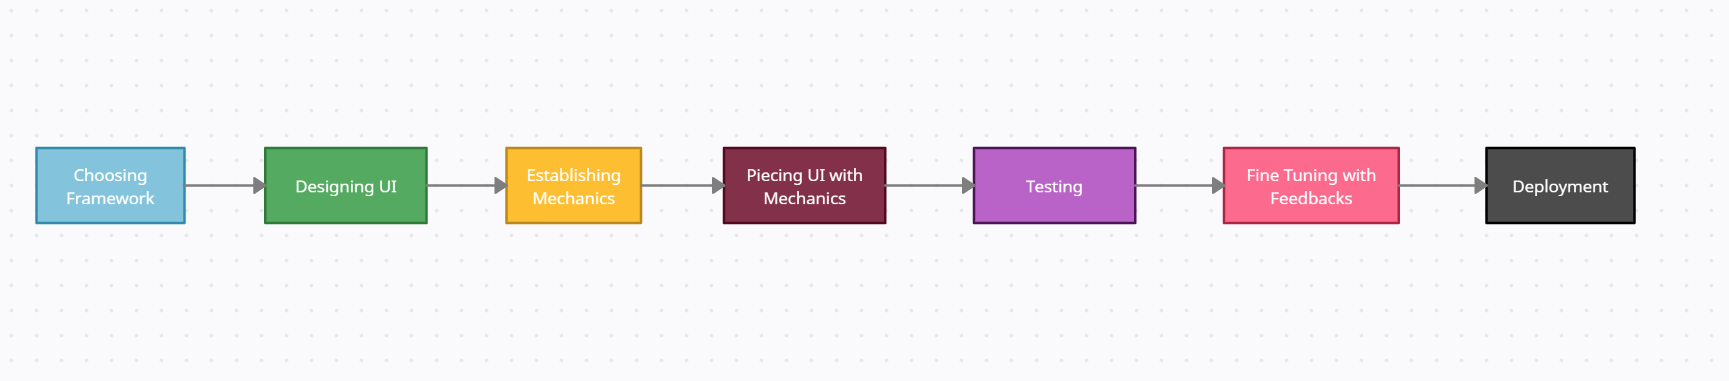
\includegraphics[scale=0.45]{SDLC.png}
   \caption{Methodologies of Problem Solving}
   \label{Methodologies of Problem Solving}
\end{figure}

1.	Choosing Framework: The process of selecting a framework for our project was a crucial step, and we carefully evaluated different options before settling on Unity. We considered the ease of adoption, the quality of the documentation, and the level of community support for each engine.
2.	Designing UI: In terms of UI design, we were fortunate to have mentors with a keen sense of aesthetics who helped us create an interface that was both intuitive and visually appealing. We took great care to ensure that the UI complemented the gameplay mechanics and enhanced the user experience.

3.	Establishing Mechanics: Developing game mechanics that were accessible to players of all ages and skill levels was one of our primary goals. We spent a significant amount of time refining and simplifying the mechanics to ensure that they were easy to understand and provided a fun and engaging experience.

4.	Piecing UI with Mechanics: The mechanics were made in isolation and the UI designed differently since, we had to piece them together that really tells us the real story of development, fun and challenging at the same time. Integrating the UI and mechanics was a challenging but rewarding process. We designed them separately, which required us to carefully consider how they would work together and make the necessary adjustments to ensure that they were seamlessly integrated.

5.	Testing: Testing in gaming is a very strenuous job since there are many scopes to test with the available limited resources we have done Playtests, Network connection testing as well making sure there is no problem in mechanics and UI.Testing and quality assurance were critical components of our development process. We conducted extensive playtests, network connection testing, and comprehensive checks of mechanics and UI to ensure that the game was polished and free of bugs and glitches.

6.	Fine Tuning with Feedbacks: The edge and boundary cases of the game had a lot of bugs which led to backtracking our mistakes and making sure it was a tight ship. We encountered several bugs during the development process that required backtracking and debugging. We listened to feedback from players and continuously refined the game to ensure an optimal experience.

7.	Deployment: Deployment for a Unity cross platform has to be done across their own respective store so, for PC it is Steam or something for Apple their App Store and Android it is Google Play Store, since we are 4 students we chose to upload our game on itch.io for deployment and uploaded binaries for each platform, we chose itch.io since it is free and a lot of indie games are there already on it. Deploying a Unity cross-platform game requires uploading it to respective stores such as Steam for PC, Apple App Store for iOS, and Google Play Store for Android. As a team of four, we chose itch.io, a free platform that hosts many indie games, to upload our game. We uploaded binaries for each platform to itch.io.

\clearpage
%end of INtroduction

%start of Literature Survey
\centering
\section{LITERATURE SURVEY}
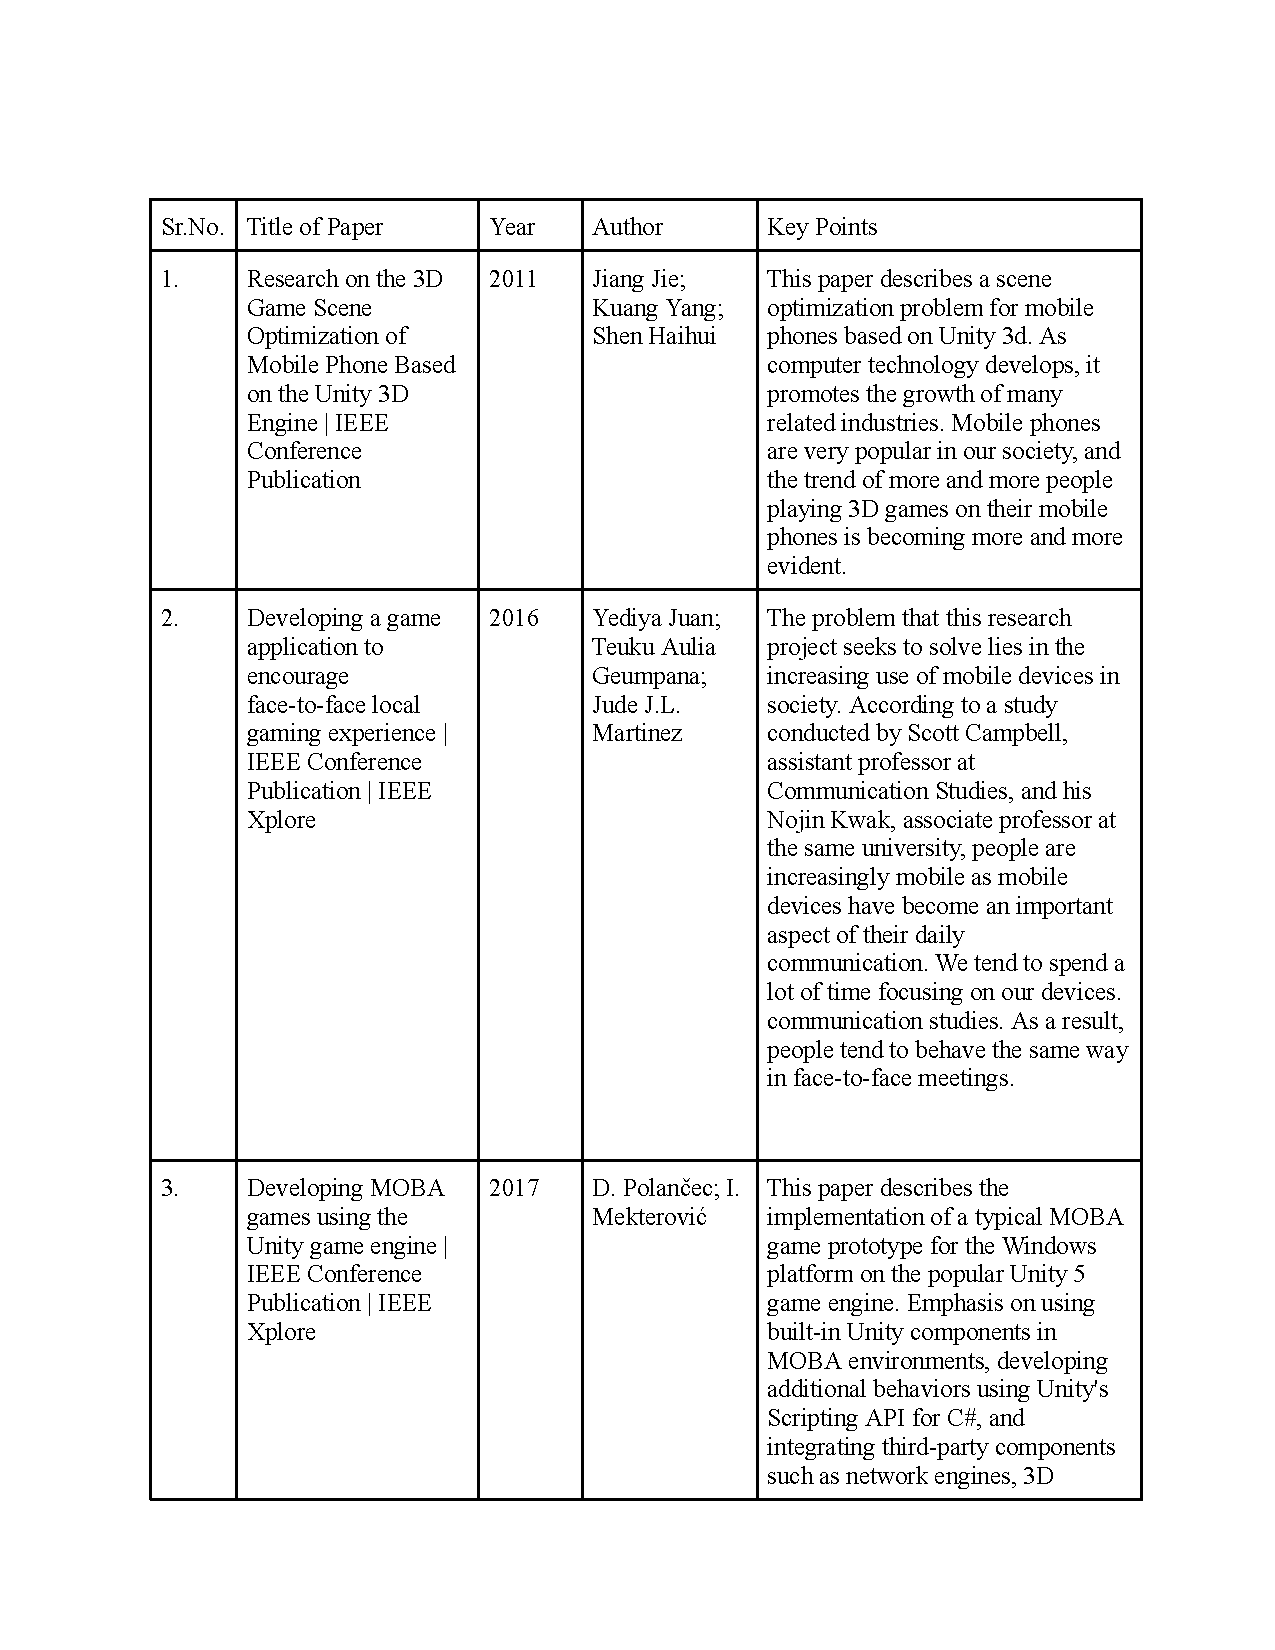
\includepdf[pages={1-} ,offset=0cm 0cm]{LitSurvey.pdf}
%end of litterature

% SOFTWARE REQUIREMENT SPECIFICATION
\centering
\section{SOFTWARE REQUIREMENT SPECIFICATION}
\raggedright
\subsection{ASSSUMPTIONS AND DEPENDENCIES}

\justifying
\setlength{\parindent}{4em}
\setlength{\parskip}{0.5em}
\renewcommand{\baselinestretch}{1.5}

\normalsize
\hspace{1.7cm}\subsubsection{Assumptions:}
\begin{itemize}\item Players are familiar with the rules of dodgeball and understand the objective of the game.
\item Players have basic knowledge of gaming controls and mechanics.
\item Players have access to the necessary equipment, such as a computer or a gaming console, to play the game.
\item The game is designed for multiplayer mode, and players can connect to the game server without any issues.
\item The game mechanics are well-defined and allow players to perform all the necessary actions to play the game effectively.
\end{itemize}

% code to fig reffrence==[figure. \ref{Simple Cryptography Process}].
\hspace{1.7cm}\subsubsection{Dependencies:}
\begin{itemize}\item Players are familiar with the rules of dodgeball and understand the objective of the game.
\item The game depends on the underlying software infrastructure, such as the operating system, web server, and database server, to function correctly.
\item The game depends on network connectivity to connect players to the game server and enable multiplayer mode.
\item The game depends on the hardware capabilities of the player's device, such as the CPU, GPU, and RAM, to run smoothly and without any lag.
\item The game depends on the availability of game assets, such as graphics, sound effects, and music, to create a rich and immersive gaming experience.
\item The game's success depends on the availability of players to participate in multiplayer mode and engage with the game.
\end{itemize}

%\textbf{Domain}: Machine Learning\\
%\textbf{Input}: Users’ Face

\centering
\raggedright
\subsection{FUNCTIONAL REQUIREMENT}

\justifying
\setlength{\parindent}{4em}
\setlength{\parskip}{0.5em}
\renewcommand{\baselinestretch}{1.5}

%\normalsize Proposed system consists of 4 modules:
\begin{itemize}\item After running the game, the UX view of the game will appear on the screen.
\item User Experience which is used to explain all aspects of a person's experience with a system.
\item The gamer can directly select "Start" from the "Main Menu"  which contains a number of Scenes like Tutorial, Matchmaking, Settings, and Quit.
\item During Tutorial and Matchmaking players can control the character and have features like pause and play and can change settings in mid-game.

\end{itemize}
\centering
\raggedright
\subsection{EXTERNAL INTERFACE REQUIREMENT}

\justifying
\setlength{\parindent}{4em}
\setlength{\parskip}{0.5em}
\renewcommand{\baselinestretch}{1.5}
%\subsubsection{ User Interface}
\normalsize\begin{itemize}\item  Maximum high regulation with minimum hardware.
\item We may provide each player with their rank.
\item Easy to operate.
\item Minimum hardware requirements which are relevant for this game.
\item Design the whole system in an efficient manner.
\end{itemize}
\subsubsection{User Interface}
%\normalsize\begin{itemize}\item   Hardware: Intel i5 Processor
%\item  Speed: 2.80 GHz
%\item  RAM: 8GB
%\item  Hard Disk: 64 GB
%\item  KeyBoard: Standard Windows Keyboard
%\end{itemize}
\subsubsection{Hardware Interfaces:}
\normalsize

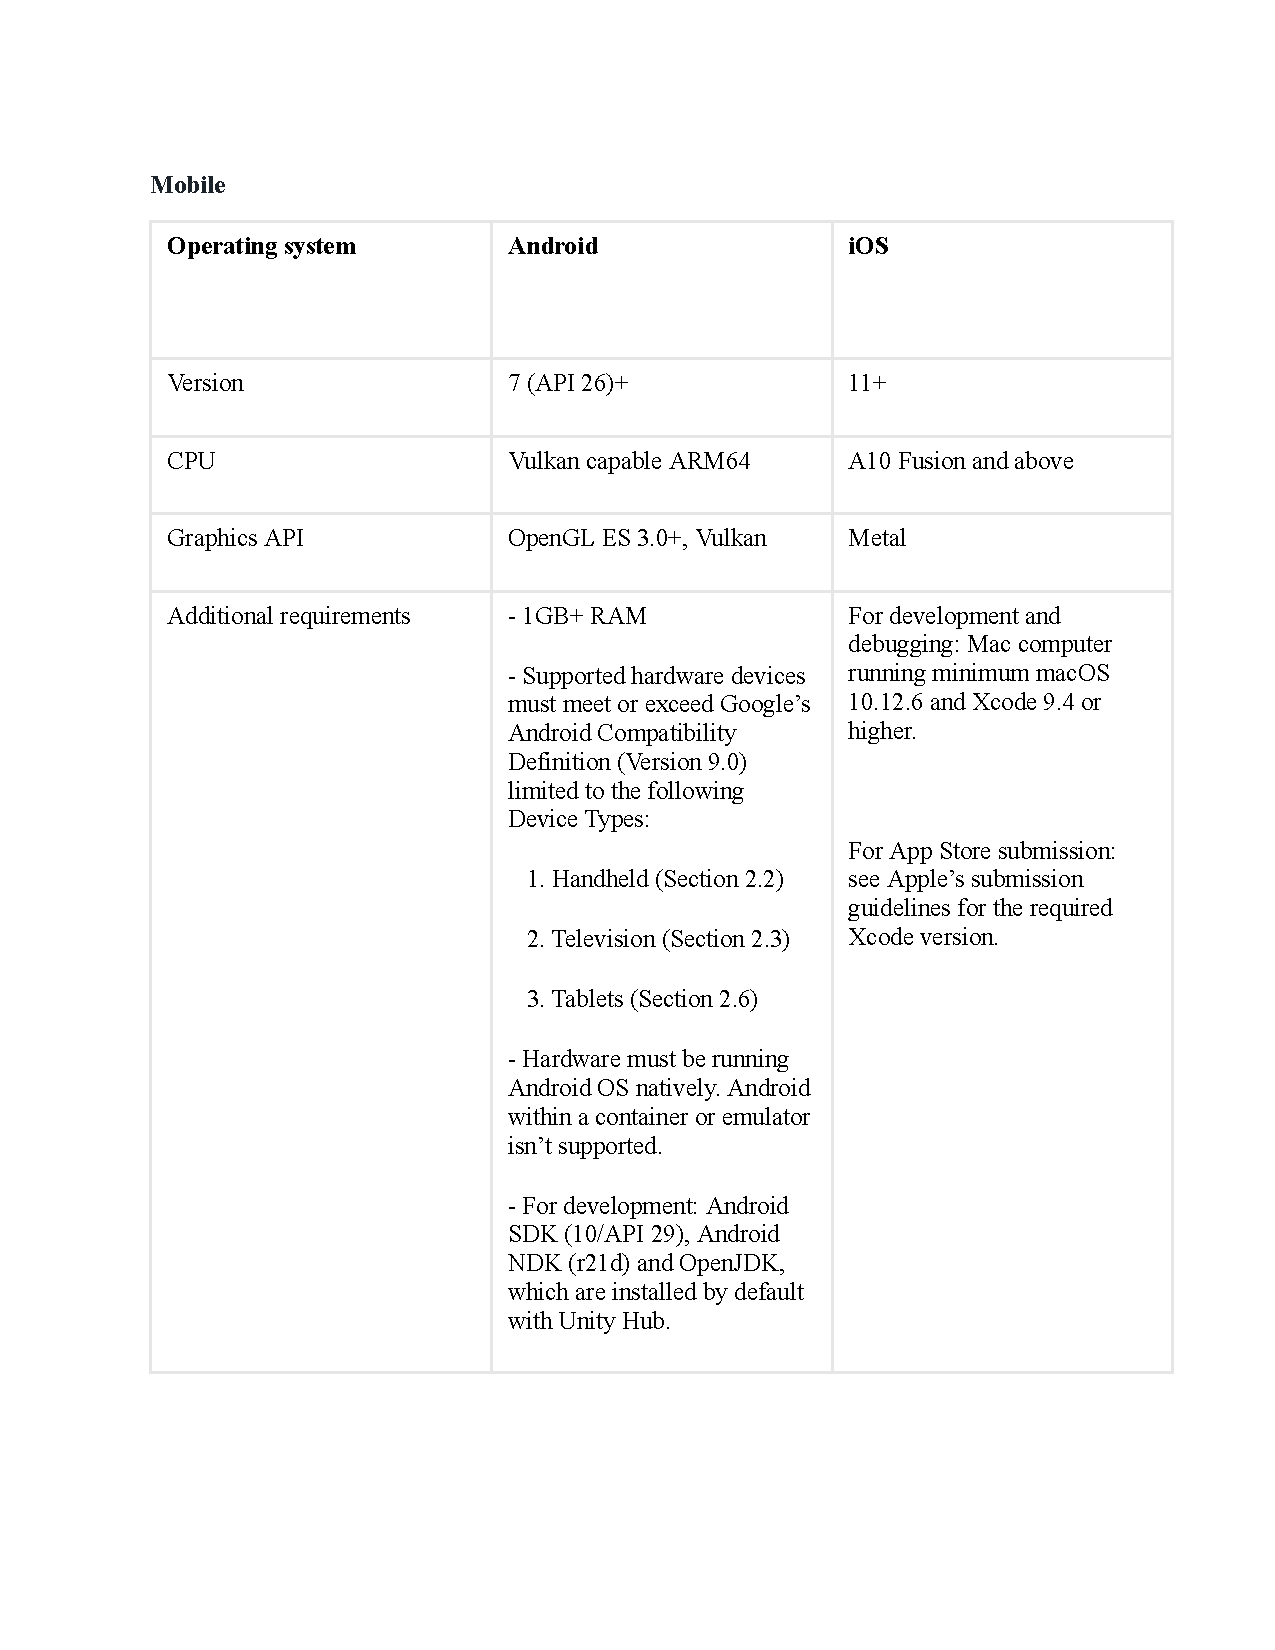
\includepdf[pages=-]{HardwareInfo.pdf}

\subsubsection{ Software Interfaces:}
\normalsize
\begin{itemize}
\item Operating System: Windows/macOS/Linux 

\item Game Engine: Unity 

\item Programming Language: C\#

\item Build Systems : .NET, Mono, Gradle, Xcode

\end{itemize}

\centering
\justifying
\setlength{\parindent}{0em}
\renewcommand{\baselinestretch}{1.5}
Unity: Unity is a cross-platform game engine developed by Unity Technologies, 
first announced and released in June 2005 at Apple Worldwide Developers Conference as a Mac OS X game engine.
The engine has since been gradually extended to support a variety of desktop, mobile, console, and virtual reality platforms.

\setlength{\parindent}{0em}
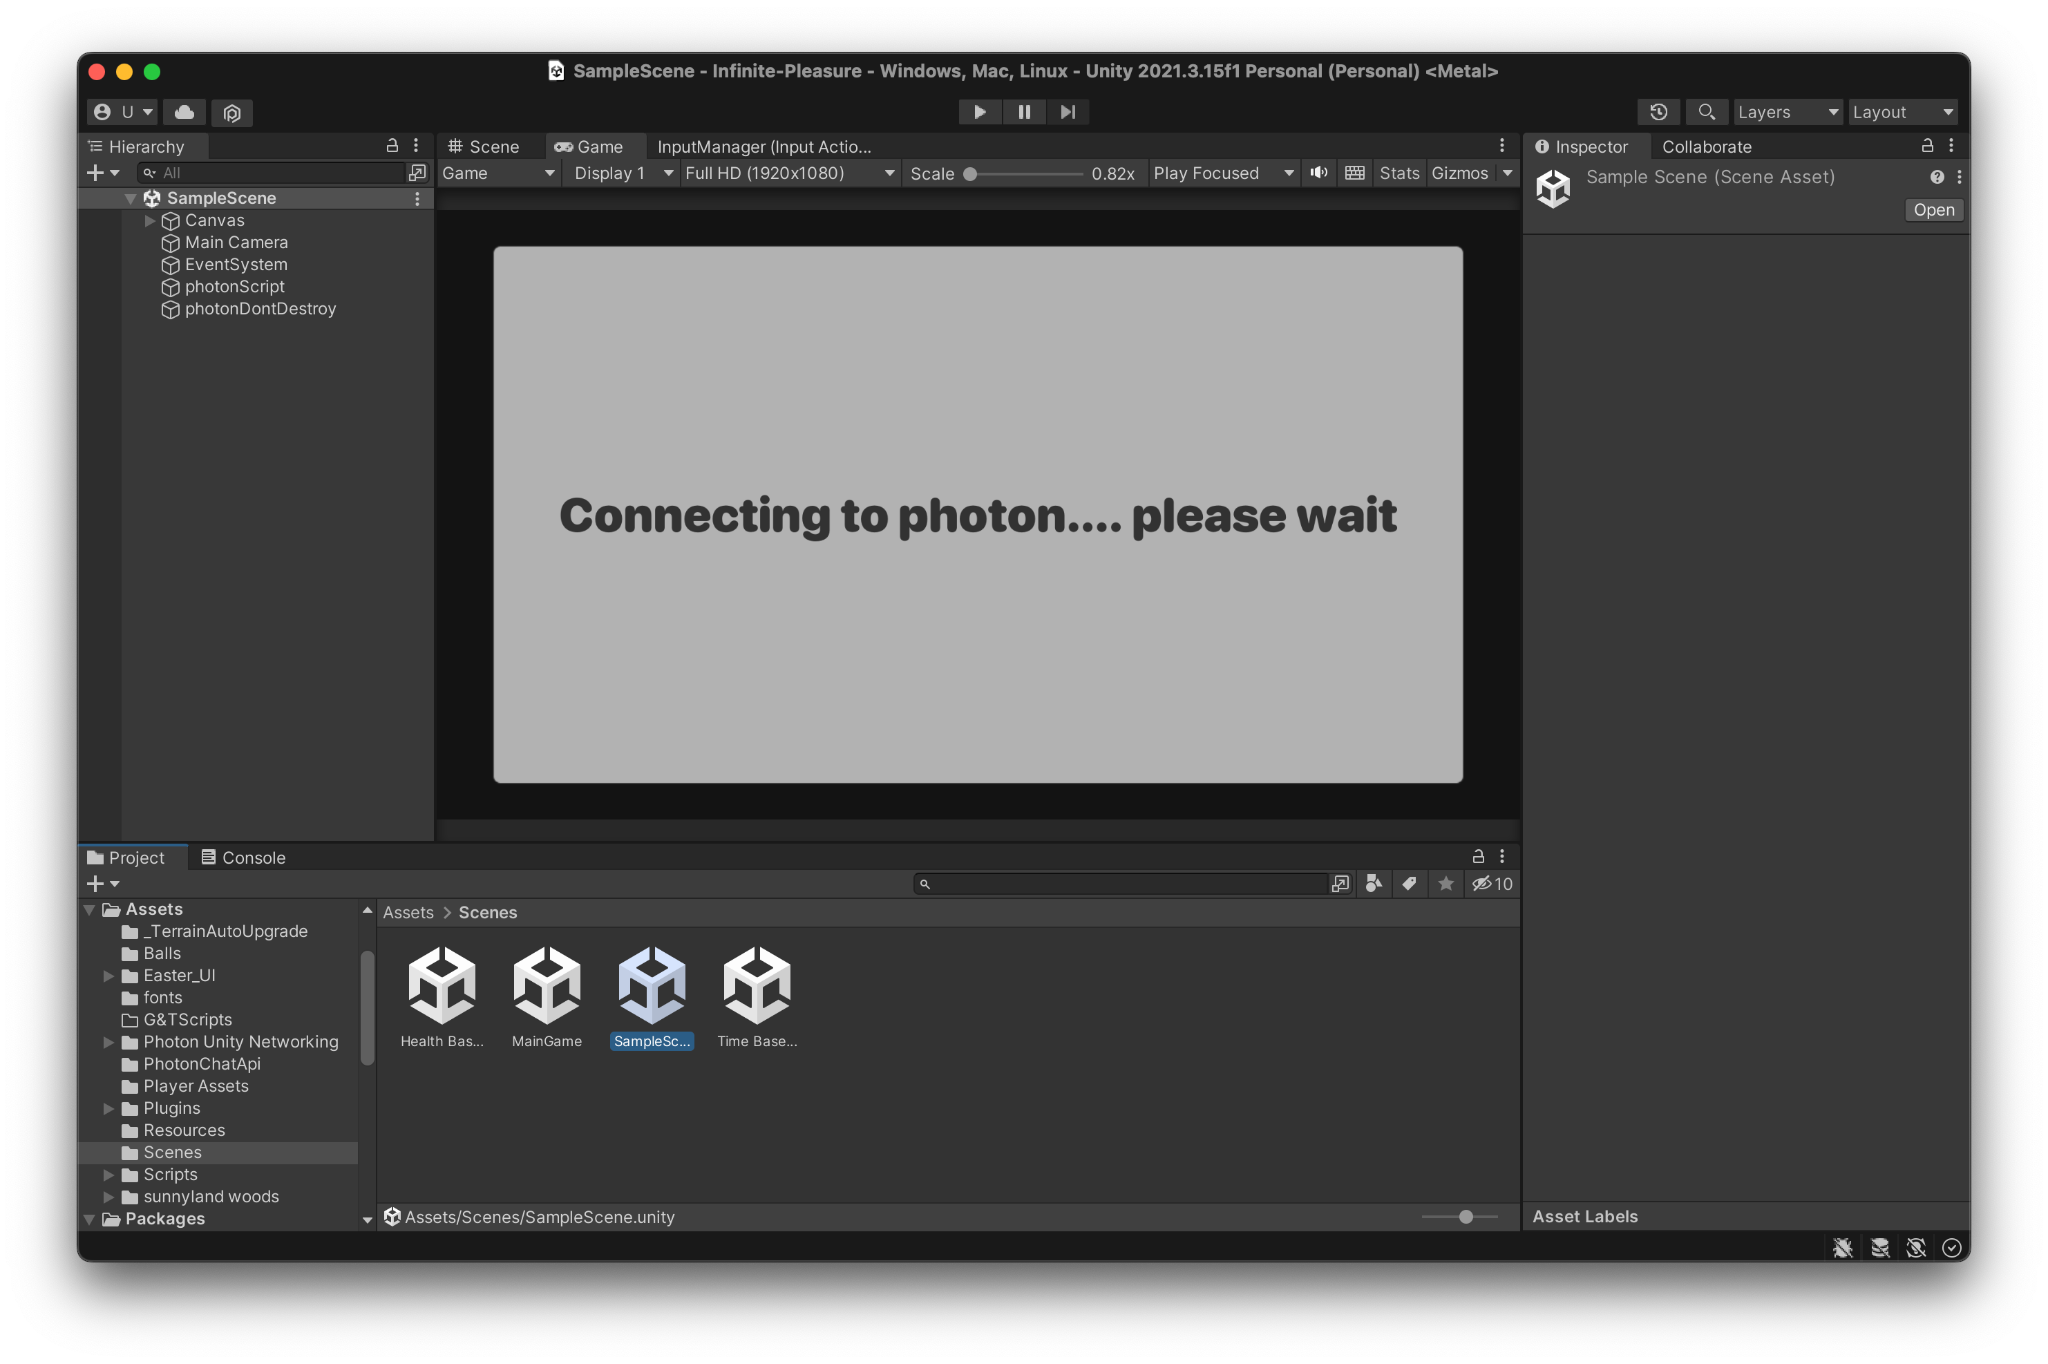
\includegraphics[scale=0.2]{Haar.png}

C-Sharp: C\# is a general-purpose, high-level multi-paradigm programming language. C\# encompasses static typing, strong typing, lexically scoped, imperative, declarative, functional, generic, object-oriented, and component-oriented programming disciplines. C-sharp (C\#) is a popular programming language developed by Microsoft in 2002. It has also been a main language for Unity game engine since 2005. Unity3D, being one of the two main obvious choices for AR/VR development, to get a handle of it if they want to develop applications with some complexity (think physics, animations, to design patterns, shaders or even sound effects).

Rider: JetBrains Rider is a fast and powerful C\# editor for Unity that runs on Windows, Mac, and Linux. With the unbeatable 2500+ smart code inspections and refactorings, Rider enhances your C\# experience, letting you write error-proof code much faster.

Visual Studio: is an integrated development environment from Microsoft.The Unity engine integrates into one unparalleled platform to create 2D and 3D games and interactive content. Create once and publish to 21 platforms, including all mobile platforms, WebGL, Mac, PC and Linux desktop, web or consoles. Visual Studio brings powerful features to C\# programmers. Write code quickly and with precision using IntelliSense. Navigate through your scripts easily and use powerful refactoring capabilities.

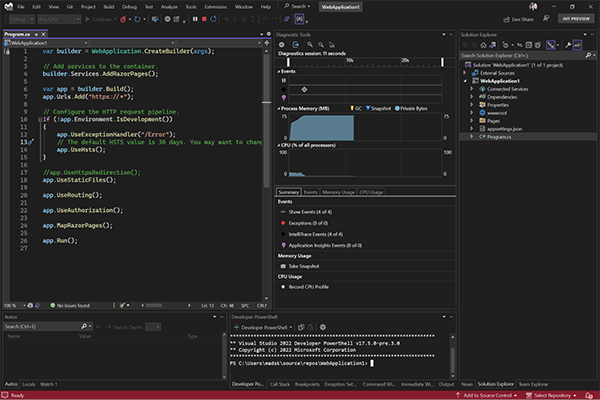
\includegraphics[scale=0.6]{image7.png}

Xcode: Xcode is Apple's integrated development environment for macOS, used to develop software for macOS, iOS, iPadOS, watchOS, and tvOS. It was initially released in late 2003; the latest stable release is version 14.1, released on November 1, 2022, via the Mac App Store with macOS Monterey. The new multi platform target creates a single interface for use across iOS, iPadOS, macOS, and tvOS. Your code is easier to maintain, and ready to be customized to take advantage of each platform’s unique capabilities.

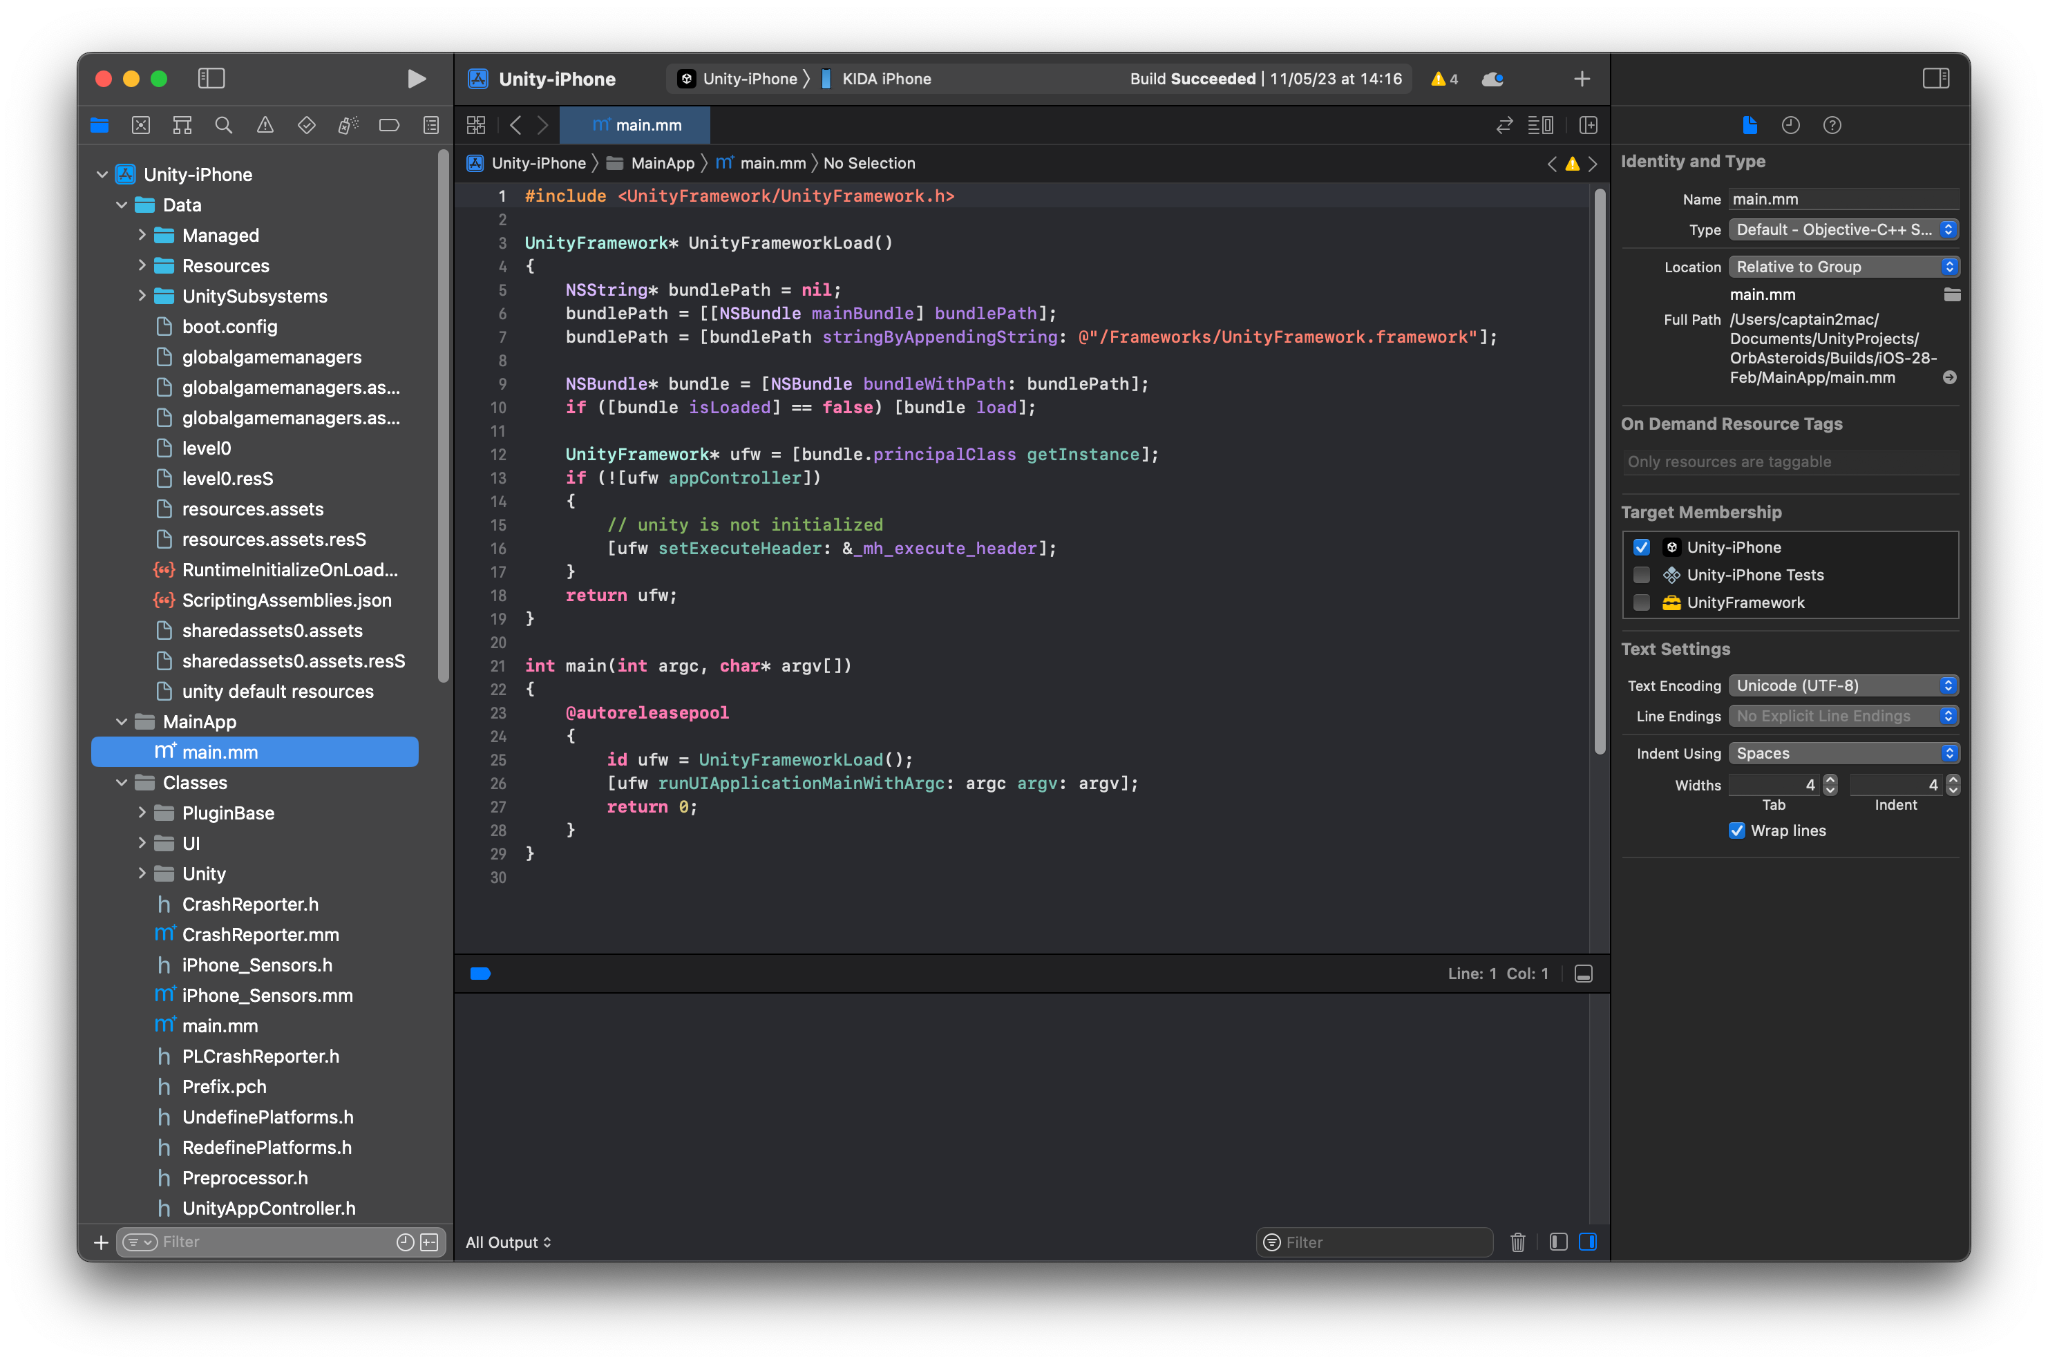
\includegraphics[scale=0.2]{image8.png}

Gradle: Gradle is a build automation tool for multi-language software development. It controls the development process in the tasks of compilation and packaging to testing, deployment, and publishing. Supported languages include Java, C/C++.

Mono: The Mono scripting backend compiles code at runtime, with a technique called just-in-time compilation (JIT). Unity uses a fork of the open source Mono project. Some platforms don’t support JIT compilation, so the Mono backend doesn’t work on every platform. Other platforms support JIT and Mono but not ahead-of-time compilation (AOT), and so can’t support the IL2CPP backend. When a platform can support both backends, Mono is the default.


\centering
\raggedright
\subsection{ NON-FUNCTIONAL REQUIREMENT}

\justifying
\setlength{\parindent}{4em}
\setlength{\parskip}{0.5em}
\renewcommand{\baselinestretch}{1.5}
\subsubsection{ Performance Requirements}
\normalsize\begin{itemize}
    \item The game will run on Android, MacOS, iOS, and Windows 10 (or newer) and requires the user to have the following components for Desktop: keyboard, mouse, monitor, and computer.
    \item The game will run with a CPU with SSE2 instruction set support and a Graphics card with DX10 (shader model 4.0) capabilities. Need a minimum of 4GB RAM, and 1GB of storage space.
    \item An Internet connection will also be required for multiplayer. The game will be running at a minimum of 1080p 60fps and a maximum of 1080p 120fps.
\end{itemize}

\subsubsection{ Safety Requirement}
\normalsize\begin{itemize}
    \item Age appropriateness: Clearly define the target audience for your game and ensure that the content, themes, and challenges are suitable for that age group. Implement age verification mechanisms if necessary.
    \item User privacy: Respect user privacy by implementing appropriate data protection measures. Clearly communicate your data collection and usage policies, and obtain user consent when necessary. Follow applicable data protection regulations, such as the General Data Protection Regulation (GDPR) if your game is available to users in the European Union.
    \item Online interactions: If your game includes online multiplayer features or chat functionality, implement measures to prevent and handle inappropriate behavior, harassment, and cyberbullying. Provide reporting and blocking mechanisms for users to address such issues.
    \item Parental controls: Consider implementing parental control features to allow parents or guardians to restrict access to certain content, set time limits, or manage in-game purchases for underage players.
    \item Game content warnings: Provide appropriate content warnings for potentially sensitive or disturbing content, such as violence, horror, or mature themes. Allow players to customize content filters if necessary.
    \item Accessibility: Ensure your game is accessible to players with disabilities. Implement features such as colorblind modes, adjustable font sizes, captioning for audio content, and support for alternative input devices.
    \item Fair gameplay: Prevent cheating, hacking, or exploiting in the game to maintain a fair and enjoyable experience for all players. Implement appropriate security measures and address any vulnerabilities promptly.
    \item Compliance with regulations: Familiarize yourself with applicable laws, regulations, and industry standards related to game safety, including consumer protection laws, advertising standards, and intellectual property rights.
    \item Apple IDFA: The Identifier for Advertisers (IDFA) is a random device identifier assigned by Apple to a user’s device. Advertisers use this to track data so they can deliver customized advertising. The IDFA is used for tracking and identifying a user (without revealing personal information).

\end{itemize}
\subsubsection{  Software Quality Attributes}

\normalsize
\begin{itemize}
    \item Usability: The game should be easy to navigate and play, with clear instructions and intuitive controls.
    \item Performance: The game should be responsive and run smoothly without any lag or glitches.
    \item Reliability: The game should function reliably and consistently without crashes or other technical issues.
    \item Maintainability: The game should be designed with maintainability in mind, with clear and well-organized code that is easy to update and modify.
    \item Security: The game should be secure, with measures in place to protect player data and prevent cheating.
    \item Scalability: The game should be able to handle a growing number of players and gameplay data without a significant decrease in performance.
    \item Compatibility: The game should be compatible with different devices, operating systems, and web browsers to reach a wider audience.
    \item Portability: The game should be easily portable between different platforms, such as mobile devices and desktop computers.
    \item Accessibility: The game should be designed to be accessible to players with different abilities, with features such as subtitles, audio descriptions, and color contrast options.
    By focusing on these software quality attributes, the 2D dodgeball game can provide a high-quality gameplay experience for players, increase engagement, and encourage repeat gameplay.
    
\end{itemize}

\centering
\raggedright
\subsection{ SYSTEM REQUIREMENTS}

\justifying
\setlength{\parindent}{4em}
\setlength{\parskip}{0.5em}
\renewcommand{\baselinestretch}{1.5}

\subsubsection{Software Requirements}

\normalsize

1. Operating System: Windows/macOS/Linux 

2. Game Engine: Unity 

3. Programming Language: C\#

Unity: Unity is a cross-platform game engine developed by Unity Technologies, first announced and released in June 2005 at Apple Worldwide Developers Conference as a Mac OS X game engine. The engine has since been gradually extended to support a variety of desktop, mobile, console, and virtual reality platforms.
The technology that we refer to as IL2CPP has two distinct parts.
An ahead-of-time (AOT) compiler
A runtime library to support the virtual machine
The AOT compiler translates Intermediate Language (IL), the low-level output from .NET compilers, to C++ source code. The runtime library provides services and abstractions like a garbage collector, platform-independent access to threads and files, and implementations of internal calls (native code which modifies managed data structures directly).
The IL2CPP AOT compiler is named il2cpp.exe. On Windows you can find it in the Editor\\Data\\il2cpp directory. On OSX it is in the Contents/Frameworks/il2cpp/build directory in the Unity installation. The il2cpp.exe utility is a managed executable, written entirely in C\#. We compile it with both .NET and Mono compilers during our development of IL2CPP.
The il2cpp.exe utility accepts managed assemblies compiled with the Mono compiler that ships with Unity and generates C++ code which we pass on to a platform-specific C++ compiler.

\subsubsection{Hardware Requirements}
\hspace{1.7cm}
The hardware requirements for a Unity dodgeball game will depend on the complexity of the game, the graphics and physics involved, and the target platform (e.g., PC, mobile, console). Here are some considerations when determining the hardware requirements:

Processor (CPU): Unity games typically rely on the CPU for gameplay and physics calculations. A multi-core processor with a higher clock speed will help handle complex calculations more efficiently.

Graphics Card (GPU): The GPU handles rendering and graphics-related tasks. A dedicated graphics card with decent performance will ensure smooth rendering and better visual quality. The specific requirements will depend on the level of graphics fidelity desired for the game.
Here are the specific requirements for different platforms:

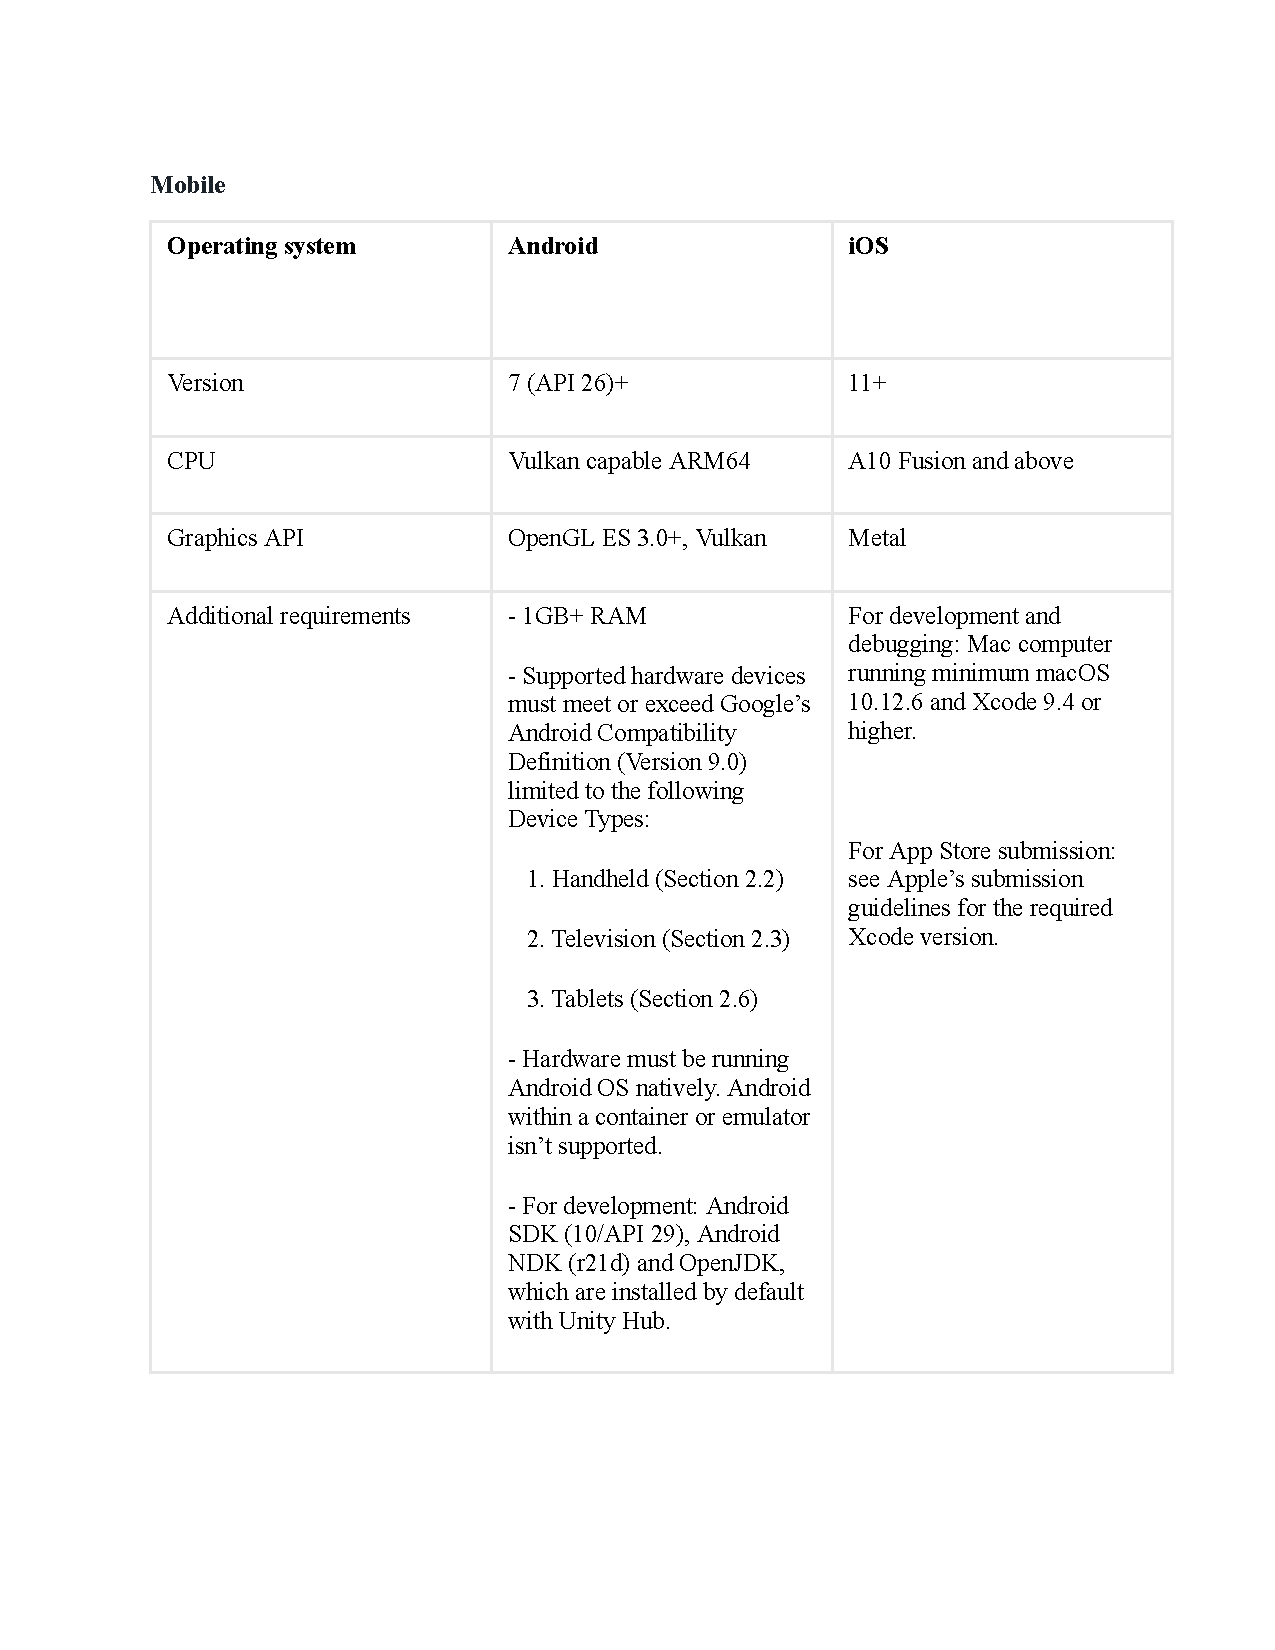
\includepdf[pages=-]{HardwareInfo.pdf}

\centering
\raggedright
\subsection{  ANALYSIS MODELS: SDLC MODEL TO BE APPLIED}

\justifying
\setlength{\parindent}{4em}
\setlength{\parskip}{0.5em}
\renewcommand{\baselinestretch}{1.5}
% \subsubsection{ User Interface}

\vspace{2cm}
\begin{figure}[h]
\centering
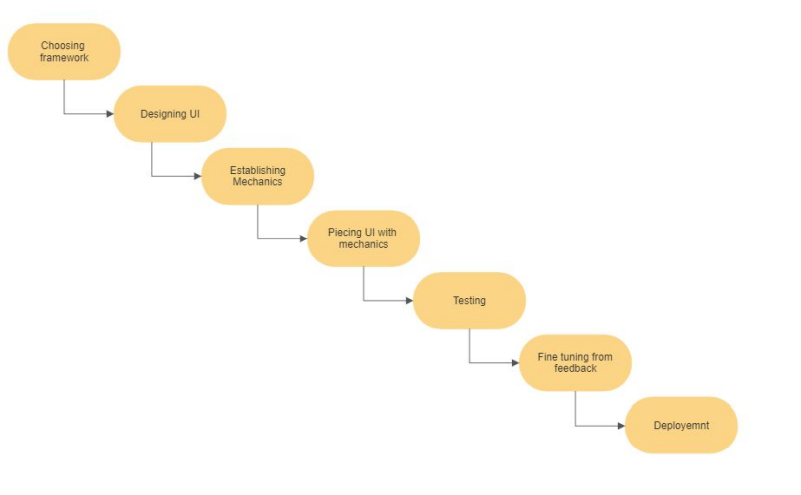
\includegraphics[scale=0.9]{Class Diagram.png}
\caption{SDLC Model}
\label{SDLC}
\end{figure}

\normalsize
SDLC Models stands for Software Development Life Cycle Models.
There are several software development life cycle (SDLC) models that can be applied in game development.
Let's take a look at a few examples:

Waterfall Model: The Waterfall Model is a linear sequential approach that involves a series of sequential phases. This model can be applied in game development by breaking down the game development process into different stages such as planning, design, implementation, testing, and maintenance. Each stage is completed before moving on to the next stage, and changes to previous stages are not allowed. This model is useful when the game requirements are well-defined and the project scope is clear.

Agile Model: The Agile Model is an iterative and incremental approach that involves continuous development and testing. This model can be applied in game development by breaking down the game development process into short development cycles called sprints. Each sprint involves designing, developing, testing, and integrating a small part of the game. The game is then tested and evaluated after each sprint, and changes are made accordingly. This model is useful when the game requirements are not well-defined, or when the project scope is subject to change.

Spiral Model: The Spiral Model is a risk-driven model that involves identifying and mitigating risks at each stage of the development process. This model can be applied in game development by breaking down the game development process into different stages, each involving risk analysis and mitigation. The game is then developed and tested, and the risks are reevaluated and mitigated in subsequent stages. This model is useful when the game requirements are not well-defined, or when the project scope is subject to change.

V-Model: The V-Model is a variation of the Waterfall Model that involves testing at each stage of the development process. This model can be applied in game development by breaking down the game development process into different stages, each involving testing and verification. The game is then developed and tested, and the testing results are used to verify and validate the game requirements. This model is useful when the game requirements are well-defined and the project scope is clear, but the testing and verification process is crucial.

Ours is:
Planning: During the planning phase, the team identifies the objectives and requirements for the game. They define the game mechanics, art style, target audience, and development timeline.

Analysis: In the analysis phase, the team evaluates the feasibility of the project and identifies potential risks. They analyze the game mechanics, UI design, and overall user experience to ensure that they meet the requirements set during the planning phase.

Design: During the design phase, the team creates detailed design documents that outline the game mechanics, level designs, and UI layout. They create wireframes, storyboards, and mockups to visualize the game design.

Development: In the development phase, the team begins coding the game using Unity. They implement the game mechanics, UI, and art assets created during the design phase. The team also conducts regular testing to identify and fix any bugs that may arise.

Testing: In the testing phase, the team conducts comprehensive testing to ensure that the game is stable, functional, and meets the user requirements. They conduct unit testing, integration testing, and acceptance testing to ensure the game is ready for release.

Deployment: During the deployment phase, the team releases the game to the appropriate platforms such as itch.io or other app stores. They ensure that the game meets the platform requirements and fix any issues that may arise during deployment.

Maintenance: After the game is released, the team continues to monitor and maintain the game to ensure it remains stable, secure, and enjoyable for players. They may release patches and updates to address bugs, improve gameplay, and add new features based on user feedback.


\clearpage
% end of SRS

%  SYSTEM DESIGN

\centering
\section{ SYSTEM DESIGN}
\raggedright
\subsection{SYSTEM ARCHITECTURE}

\justifying
\setlength{\parindent}{0em}
\setlength{\parskip}{0em}
\renewcommand{\baselinestretch}{1.5}

\vspace{0.5cm}
\begin{figure}[h]
\centering
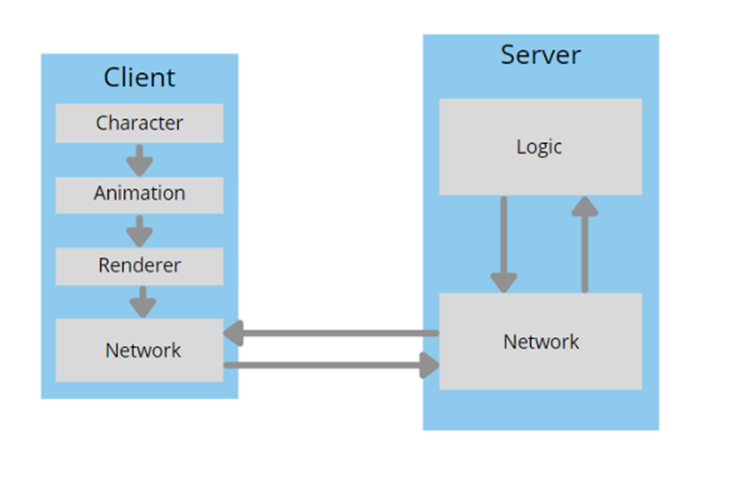
\includegraphics[scale=0.7]{Data Flow diagram-0.png}
\caption{ System Architecture}
\label{ System Architecture}
\end{figure}
\vspace{0.1cm}

\raggedright
\subsection{UML DIAGRAMS}

\justifying
\setlength{\parindent}{4em}
\setlength{\parskip}{0.5em}
\renewcommand{\baselinestretch}{1.5}
\normalsize
\subsection{CLASS DIAGRAM}
Class diagram describes the structure of a system by showing the system’s classes, Their
attributes, and the relationships among the classes. Proposed system contains five different 
types of classes and each posses their own attributes and methods. Main Classes of the 
proposed system are NDSRRC, FP Tree, Apriory, Sanitised DB each have different 
functionalities.
\setlength{\parindent}{0em}
\setlength{\parskip}{0em}
\begin{figure}[h]
\centering
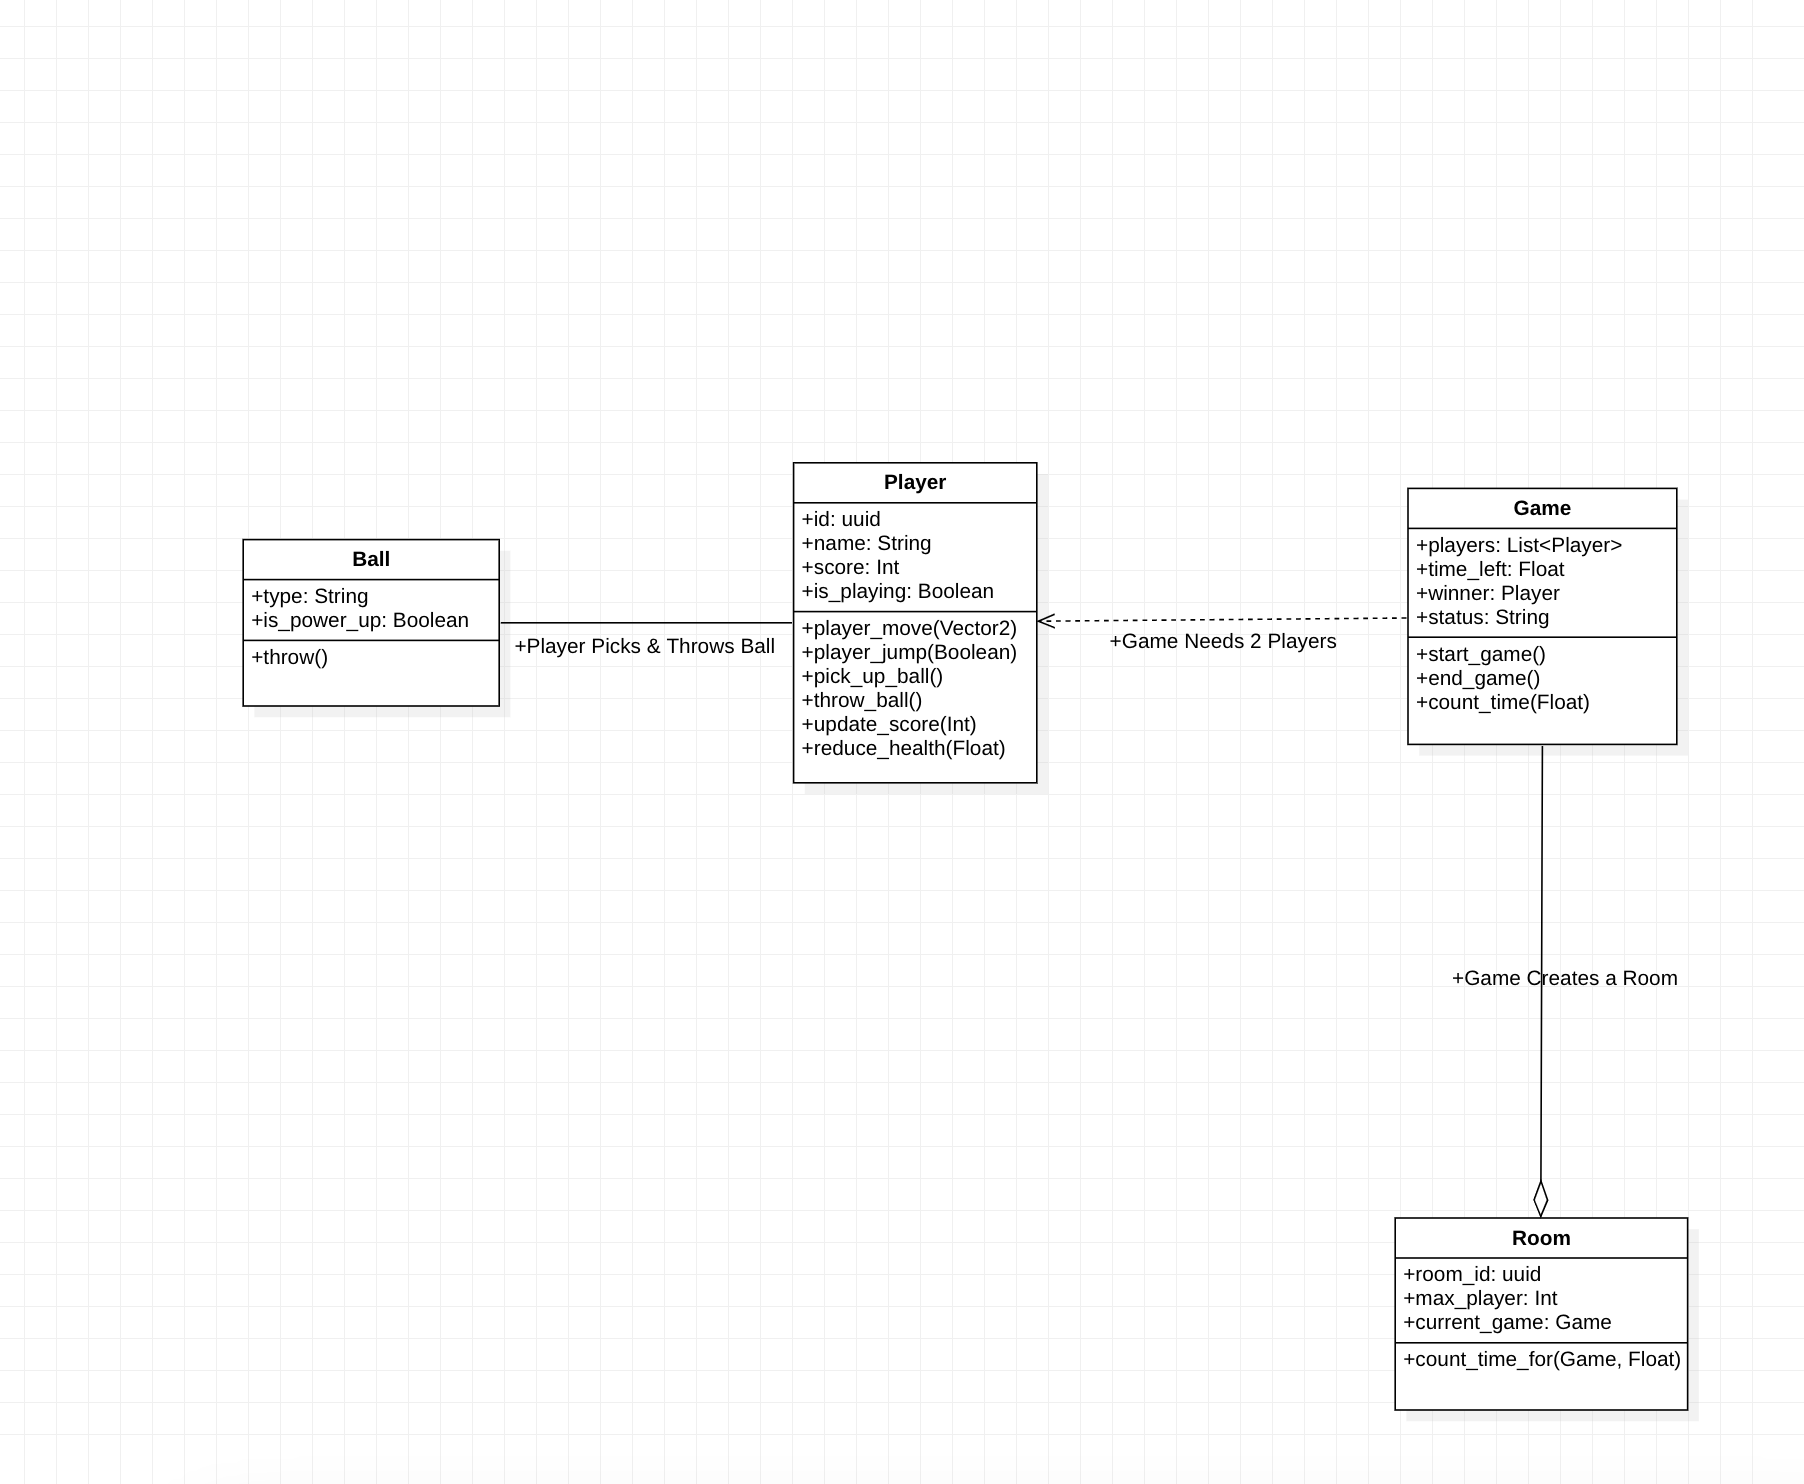
\includegraphics[scale=0.5]{Class.png}
\caption{ Class Diagram}
\label{ Class Diagram}
\end{figure}

\clearpage

\justifying
\setlength{\parindent}{4em}
\setlength{\parskip}{0.5em}
\renewcommand{\baselinestretch}{1.5}
\normalsize
\subsection{ACTIVITY DIAGRAM}
An activity is particular operation of the system. An activity diagram is intended to represent
stepwise work-flow of activities or actions that can take place in the system. It shows overall
flow of control and models computational and organizational processes. Activity diagrams
are used to model dynamic aspects of the system. 
\setlength{\parindent}{0em}
\setlength{\parskip}{0em}
\begin{figure}[h]
\centering
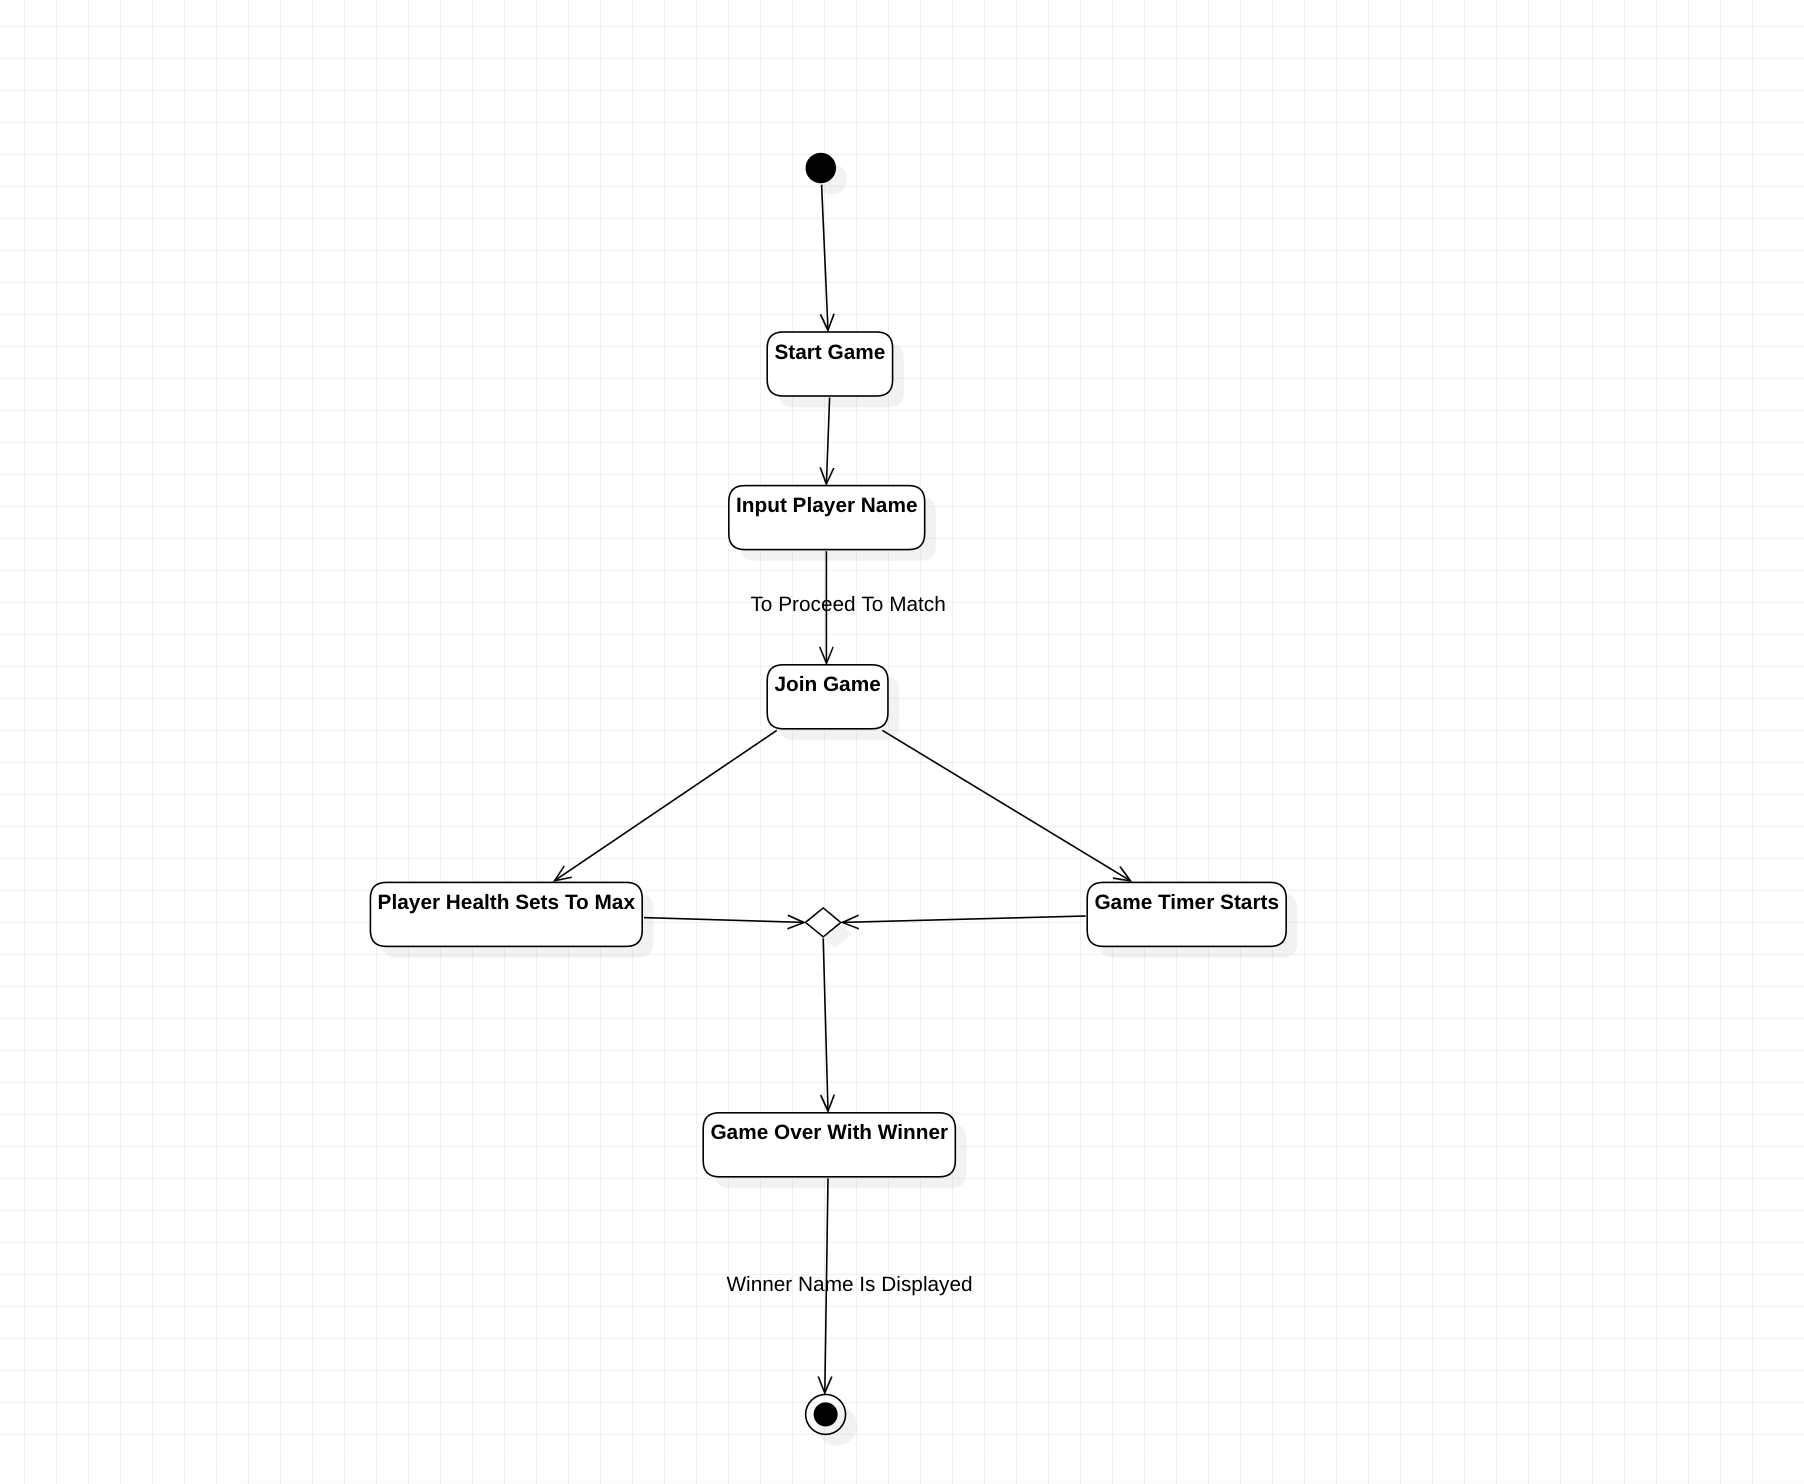
\includegraphics[scale=0.42]{Activity.png}
\caption{ Activity Diagram}
\label{ Activity Diagram}
\end{figure}

\clearpage

\justifying
\setlength{\parindent}{4em}
\setlength{\parskip}{0.5em}
\renewcommand{\baselinestretch}{1.5}
\normalsize
\subsection{USE CASE DIAGRAM}
A use case diagram in the Unified Modelling Language (UML) is a type of behavioral
diagram defined by and created from a Use-case analysis. Its purpose is to present a graphical 
overview of the functionality provided by a system in terms of actors, their goals 
(represented as use cases), and any dependencies between those use cases. The main purpose 
of a use case diagram is to show what system functions are performed for which actor. Roles 
of the actors in the system can be depicted.
\setlength{\parindent}{0em}
\setlength{\parskip}{0em}
\begin{figure}[h]
\centering
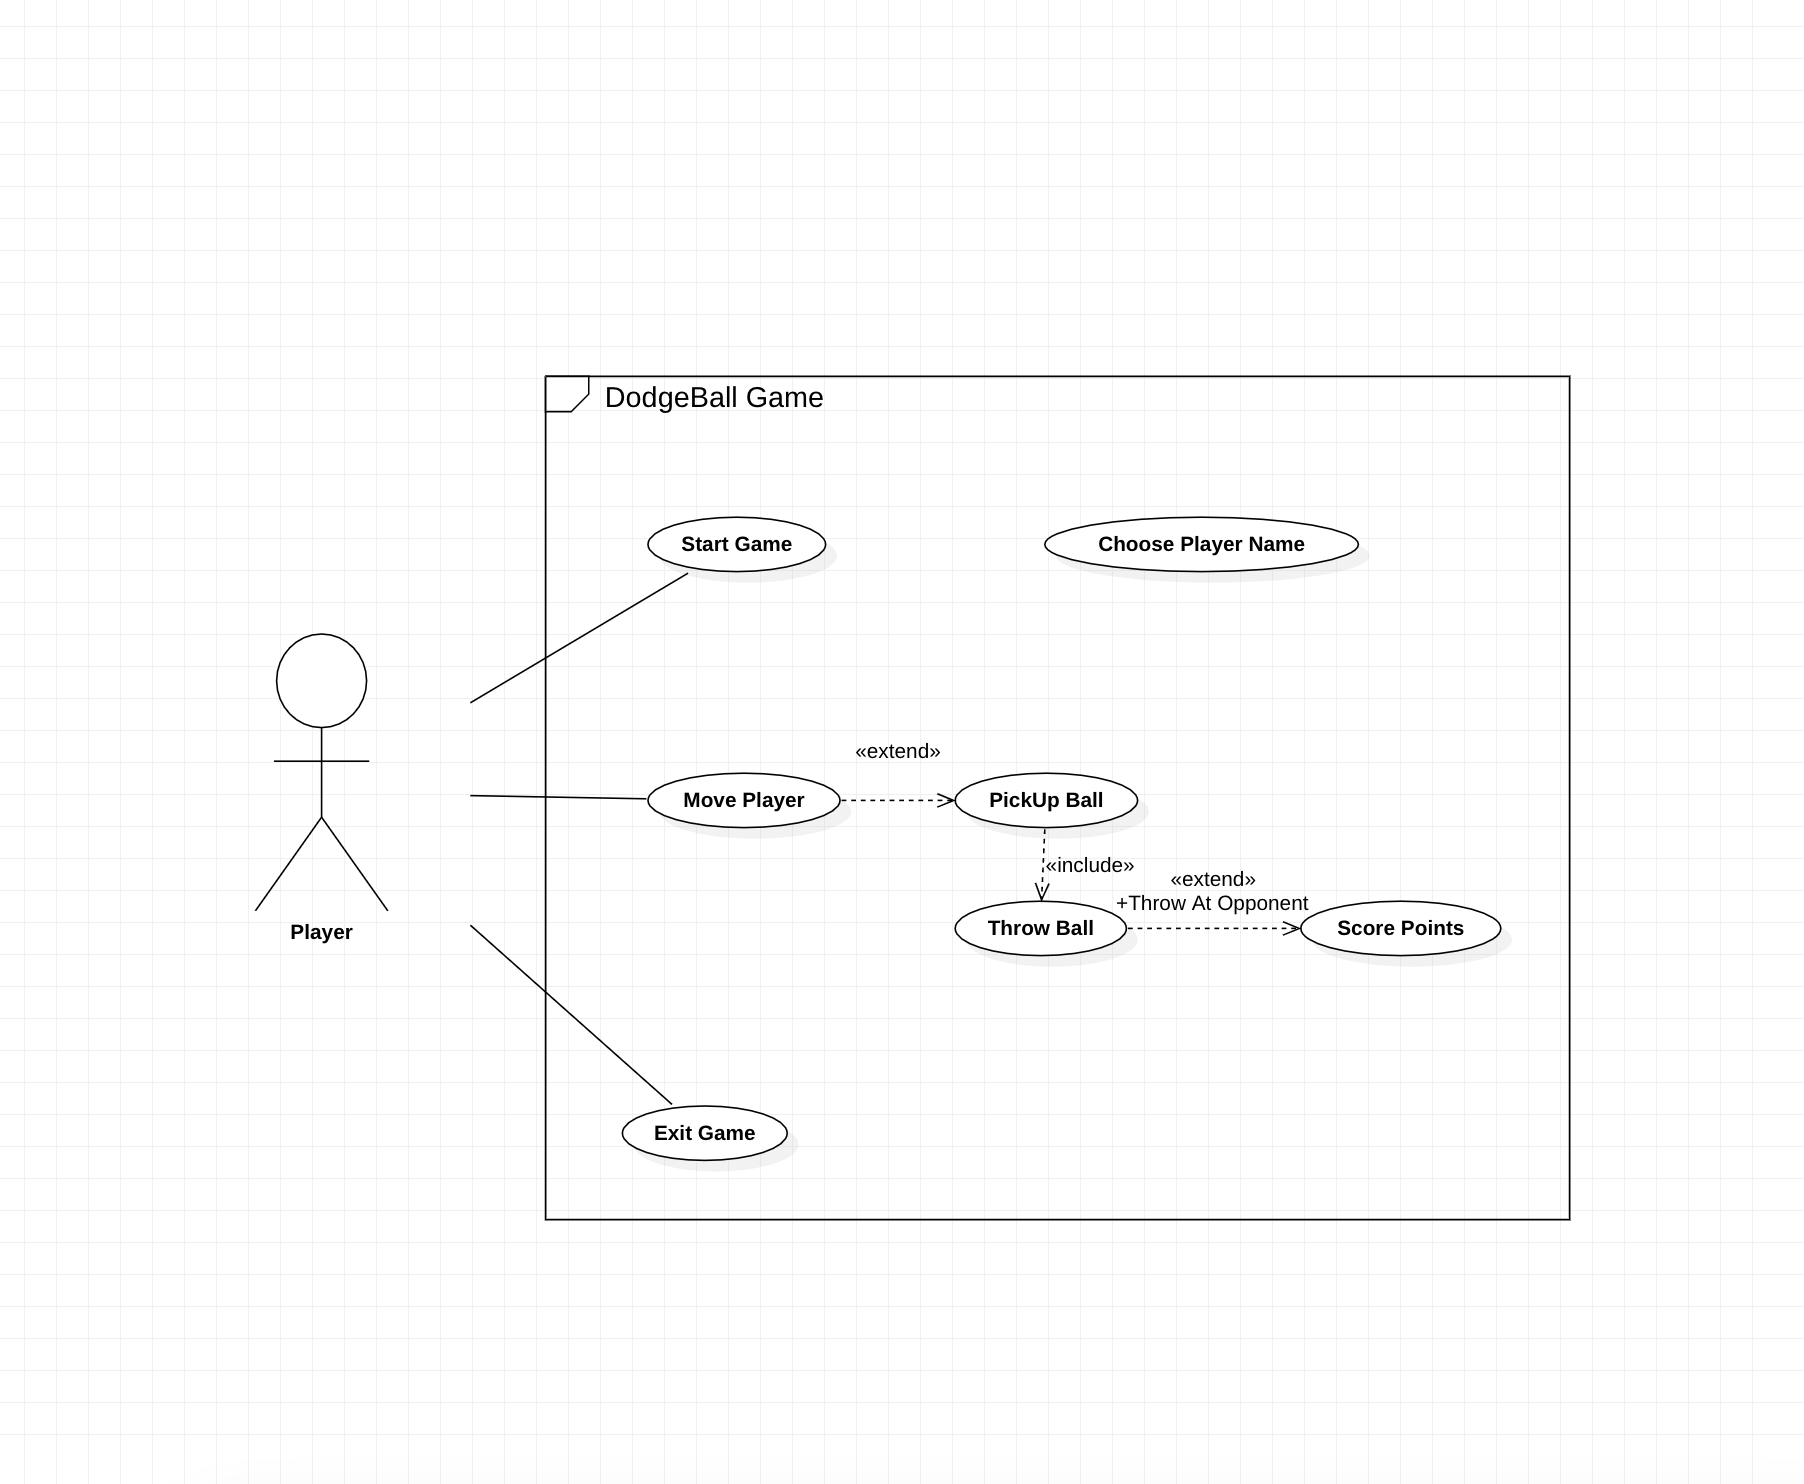
\includegraphics[scale=0.42]{Use case.png}
\caption{ Use Case Diagram}
\label{ Use Case Diagram}
\end{figure}

\clearpage

\large\textbf{MATHEMATICAL MODEL}
\normalsize
\justifying
\setlength{\parindent}{4em}
\setlength{\parskip}{0.5em}
\renewcommand{\baselinestretch}{1.5}
\vspace{0.1cm}
\begin{enumerate}
\item Player positions:
Let P1(x1, y1) and P2(x2, y2) represent the positions of Player 1 and Player 2 on a 2D plane.

\item Position and Velocity:
Let B(x, y) represent the position of the ball on the 2D plane.
Let Vx and Vy represent the ball's velocity components in the x and y directions.

\item Player movement:
Players can move in the x and y directions. Let $\Delta\mathrm{R}$x1, $\Delta\mathrm{R}$y1, $\Delta\mathrm{R}$x2, and $\Delta\mathrm{R}$y2 represent the changes in position for Player 1 and Player 2, respectively.
P1\_new(x1 + $\Delta\mathrm{R}$x1, y1 + $\Delta\mathrm{R}$y1) and P2\_new(x2 + $\Delta\mathrm{R}$x2, y2 + $\Delta\mathrm{R}$y2) represent the new positions of Player 1 and Player 2 after movement.

\item Ball movement:
The ball's position changes based on its velocity: B\_new(x + Vx * t, y + Vy * t), where t is the time elapsed since the last position update.

\item Throwing the ball:
When a player throws the ball, the ball's velocity components (Vx, Vy) are updated based on the throw's direction and strength.

\item Collision detection:
To determine if the ball hits a player, calculate the distance between the ball and each player using the Euclidean distance formula: d = sqrt((x2 - x1)\^2 + (y2 - y1)\^2).
If the distance is less than or equal to a predefined threshold (e.g., the sum of the player's and ball's radii), the player is considered hit.

\item Scoring and game state:
When a player is hit, the opposing player scores a point.
The game continues until a predefined number of points are scored by one of the players, or a time limit is reached.


\end{enumerate}
%end of design


\clearpage

\centering
\section{PROJECT PLAN}
\justifying
\setlength{\parindent}{4em}
\setlength{\parskip}{0.5em}
\renewcommand{\baselinestretch}{1.5}

%\normalsize In this chapter we are going to have an overview about how much time does it took to complete each task like- Preliminary Survey Introduction and Problem Statement, Literature Survey, Project Statement, Software Requirement and Specification, System Design, Partial Report Submission, Architecture Design, Implementation, Deployment, Testing, Paper Publish, Report Sub- mission and etcetera. This chapter also focuses on the stakeholder list which gives information about project type, customer of the proposed system, user and project member who developed the system.
\subsection{PROJECT ESTIMATE}
\subsubsection{Hardware Cost}

\begin{itemize}
\item Laptop Cost: Rs 2,35,001.00
\item Controller:  Rs 2,199.00
\end{itemize}
Laptop Used 
\begin{itemize}
\item Asus ROG:
\begin{itemize}
\item Processor: AMD  Ryzen 9 5000 series
\item GPU: Nvidia RTX GeForce 3050
\end{itemize}
\item MacBook Pro (M1) 
\end{itemize}


\subsubsection{Software Cost}
\justifying
\setlength{\parindent}{4em}
\setlength{\parskip}{0.5em}
\renewcommand{\baselinestretch}{1.5}
\vspace{0.1cm}
\begin{itemize}
\item Unity License:   Rs 1,80,000.00
\item Apple Developer License: \$ 99.00
\item Google Developer License: \$ 9.00
\item JetBrains Rider License: \$ 349.00
\end{itemize}

\subsubsection{Other Cost}
\justifying
\setlength{\parindent}{4em}
\setlength{\parskip}{0.5em}
\renewcommand{\baselinestretch}{1.5}
\vspace{0.1cm}
\begin{itemize}
\item Unity Asset
\begin{itemize}
\item Animated Characters: 34.99 Dollars
\item Photon Networking: 99 Dollars
\item Royalty free:  1.99 Dollars
\end{itemize}
\end{itemize}

\subsection{RISK MANAGEMENT}
\justifying
\setlength{\parindent}{4em}
\setlength{\parskip}{0.5em}
\renewcommand{\baselinestretch}{1.5}
\vspace{0.1cm}

\subsubsection{Risk Identification And Risk Analysis}
\justifying
\setlength{\parindent}{2em}
\setlength{\parskip}{0.5em}
\renewcommand{\baselinestretch}{1.5}
\vspace{0.1cm}
\normalsize
Developing a dodgeball game using Unity can pose several risks, which the development team needs to manage to ensure project success. Here are some potential risks and their corresponding risk management strategies:

Technical Risks: There are risks associated with the technical aspects of developing a game, such as software and hardware failures, bugs, and compatibility issues. To manage these risks, the development team should implement a robust quality assurance and testing process, conduct regular code reviews, and maintain a backup plan in case of unforeseen technical issues. The team should also keep up-to-date with the latest Unity updates and patches to minimize the risk of compatibility issues.

Scope Creep: As the development process progresses, there may be a tendency to add additional features and functionality to the game, leading to scope creep. To manage this risk, the development team should establish a clear scope of work and requirements document at the outset of the project and strictly adhere to it. Any changes to the scope should be carefully evaluated and approved before implementation. The team should also maintain effective communication with stakeholders to ensure that their expectations are aligned with the project scope.

Resource Constraints: Developing a game requires significant resources, including time, money, and talent. To manage the risk of resource constraints, the development team should carefully evaluate available resources and allocate them efficiently. This may involve prioritizing tasks, outsourcing certain functions, or seeking additional funding or talent. The team should also maintain a contingency plan in case of unforeseen resource constraints.

User Acceptance: Ultimately, the success of a game depends on its acceptance by the end-users. To manage the risk of user acceptance, the development team should conduct market research to understand user preferences and expectations, engage in regular user testing and feedback, and implement changes based on user feedback. The team should also consider incorporating analytics tools to gather data on user engagement and behavior.

Legal Risks: Developing a game can also expose the development team to legal risks, such as copyright infringement, trademark violations, and data privacy breaches. To manage these risks, the development team should conduct regular legal reviews, adhere to industry standards and regulations, and maintain appropriate data protection measures. The team should also ensure that all game assets, including art, music, and sound effects, are legally acquired or licensed.

\subsubsection{Overview of Risk Mitigation, Monitoring, Management}
\justifying
\setlength{\parindent}{4em}
\setlength{\parskip}{0.5em}
\renewcommand{\baselinestretch}{1.5}

\normalsize
\textbf{Risk Mitigation:} \newline
Technical Risks: To mitigate technical risks, the development team should establish a robust quality assurance and testing process, conduct regular code reviews, and maintain a backup plan in case of unforeseen technical issues.
Scope Creep: To mitigate scope creep, the development team should establish a clear scope of work and requirements document at the outset of the project and strictly adhere to it. Any changes to the scope should be carefully evaluated and approved before implementation.
Resource Constraints: To mitigate the risk of resource constraints, the development team should carefully evaluate available resources and allocate them efficiently. This may involve prioritizing tasks, outsourcing certain functions, or seeking additional funding or talent.
User Acceptance: To mitigate the risk of user acceptance, the development team should conduct market research to understand user preferences and expectations, engage in regular user testing and feedback, and implement changes based on user feedback.
Legal Risks: To mitigate legal risks, the development team should conduct regular legal reviews, adhere to industry standards and regulations, and maintain appropriate data protection measures.\newline
\textbf{Risk Monitoring:}\newline
The development team should regularly monitor risks and their potential impact on the project. This may involve conducting regular risk assessments and updating the risk management plan accordingly.\newline
\textbf{Risk Management:}\newline
The development team should have a clear risk management plan in place that outlines the steps to be taken in the event of a risk materializing. This may involve contingency planning, risk transfer, or risk acceptance.
Overall, risk mitigation, monitoring, and management are essential for the successful development and deployment of your game. By identifying potential risks and implementing strategies to mitigate them, your team can ensure a smooth and efficient development process, leading to a successful and well-received game.


\subsection{PROJECT SCHEDULE}

\justifying
\setlength{\parindent}{4em}
\setlength{\parskip}{0.5em}
\renewcommand{\baselinestretch}{1.5}
\hspace{1.5cm} Creating a project schedule for a game development using Unity for a dodgeball game can be a complex task as it depends on various factors such as the game's scope, the number of features, the size of the development team, and the available resources. 
\begin{enumerate} 
\item Planning phase (2 weeks)
\begin{itemize}
\item Define project scope, requirements, and goals
\item Create a detailed project plan and schedule
\item Identify necessary resources and allocate them accordingly
\item Set up communication channels and reporting mechanisms
\end{itemize}
\item Design phase (4 weeks)
\begin{itemize}
\item Create game design documents including the game mechanics, UI/UX, levels, and characters
\item Develop the game's art style, visual design, and audio design
\item Conduct internal reviews and get feedback from stakeholders
\end{itemize}
\item Development phase (7 weeks)
\begin{itemize}
\item Develop the game mechanics using Unity, including player movement, ball physics, and collision detection
\item Implement the UI/UX design, including menus, HUD, and feedback elements
\item Develop levels and environments, and design AI opponents
\item Conduct regular testing and debugging, and refine the game mechanics and design based on feedback
\end{itemize}
\item Quality assurance and testing phase (2 weeks)
\begin{itemize}
\item Conduct rigorous testing on multiple platforms and devices
\item Identify and resolve bugs and issues
\item Conduct user testing and incorporate feedback
\end{itemize}
\item Deployment and launch phase (2 weeks)
\begin{itemize}
\item Prepare the game for deployment on various platforms, including Steam, App Store, and Google Play Store
\item Develop marketing and promotional materials
\item Launch the game and monitor user feedback
\end{itemize}
\end{enumerate}
It's important to note that this is just an example project schedule and can vary depending on the project's specific requirements of the available resources.

\subsection{TEAM ORGANIZATION}
\subsubsection{Team Structure}

 1.  Team Members
\begin{itemize}
\item Ankur Patil
\item Lalu Nair
\item Sharan Thakur
\item Viren Patil
\end{itemize}
2.  Project Guide
\begin{itemize}
\item Guide: Asst. Prof. Sharad Adsure 
\item Co Guide : Asst. Prof. Deepika Jaiswal  
\end{itemize}
3.  Company Guide
\begin{itemize}
\item Mr. Varun Mehta (CTO) 
\item Mr. Avnish Oswal (Sr. Software Engineer)
\end{itemize}

\subsubsection{Team Management Reporting And Communication}
\justifying
\setlength{\parindent}{2em}
\setlength{\parskip}{0.5em}

In our company, we were fortunate to have a mentor named Varun who played an essential role in our project development process. Varun would assign tasks to the team, taking into account each member's skill set and experience level. He provided clear and concise instructions for each task and ensured that we understood the requirements before starting work.

During the task execution, the team would frequently face questions and doubts about the task requirements. In such instances, we would seek help from another mentor, Avnish, who was readily available to clarify any uncertainties and provide guidance on best practices. Once we had a better understanding of the task requirements, we would start working on it.

After the task completion, we would submit our work to Avnish for review. Avnish would evaluate our output and provide us with feedback on areas of improvement or potential issues. We would then use this feedback to refine and improve our work.

Once we had addressed the feedback, Varun would review our completed task to ensure that it met the project's quality standards. If there were any shortcomings, he would inform us, and we would work to rectify them. Once the task met the project's standards, we would proceed to the next task assigned by Varun.

In summary, our company had a well-defined process for task assignment, execution, feedback incorporation, and review. This process helped us ensure that our work met the project's quality standards and contributed to a successful outcome.

\clearpage


\centering


\centering
\section{RESULT}

\justifying
\setlength{\parindent}{4em}
\setlength{\parskip}{0.5em}
\renewcommand{\baselinestretch}{1.5}
\vspace{1cm}
\subsection{SCREENSHOTS}
\textbf{Game UI}


\begin{center}

\includegraphics[scale=0.2]{image20.png}
\label{Game UI}
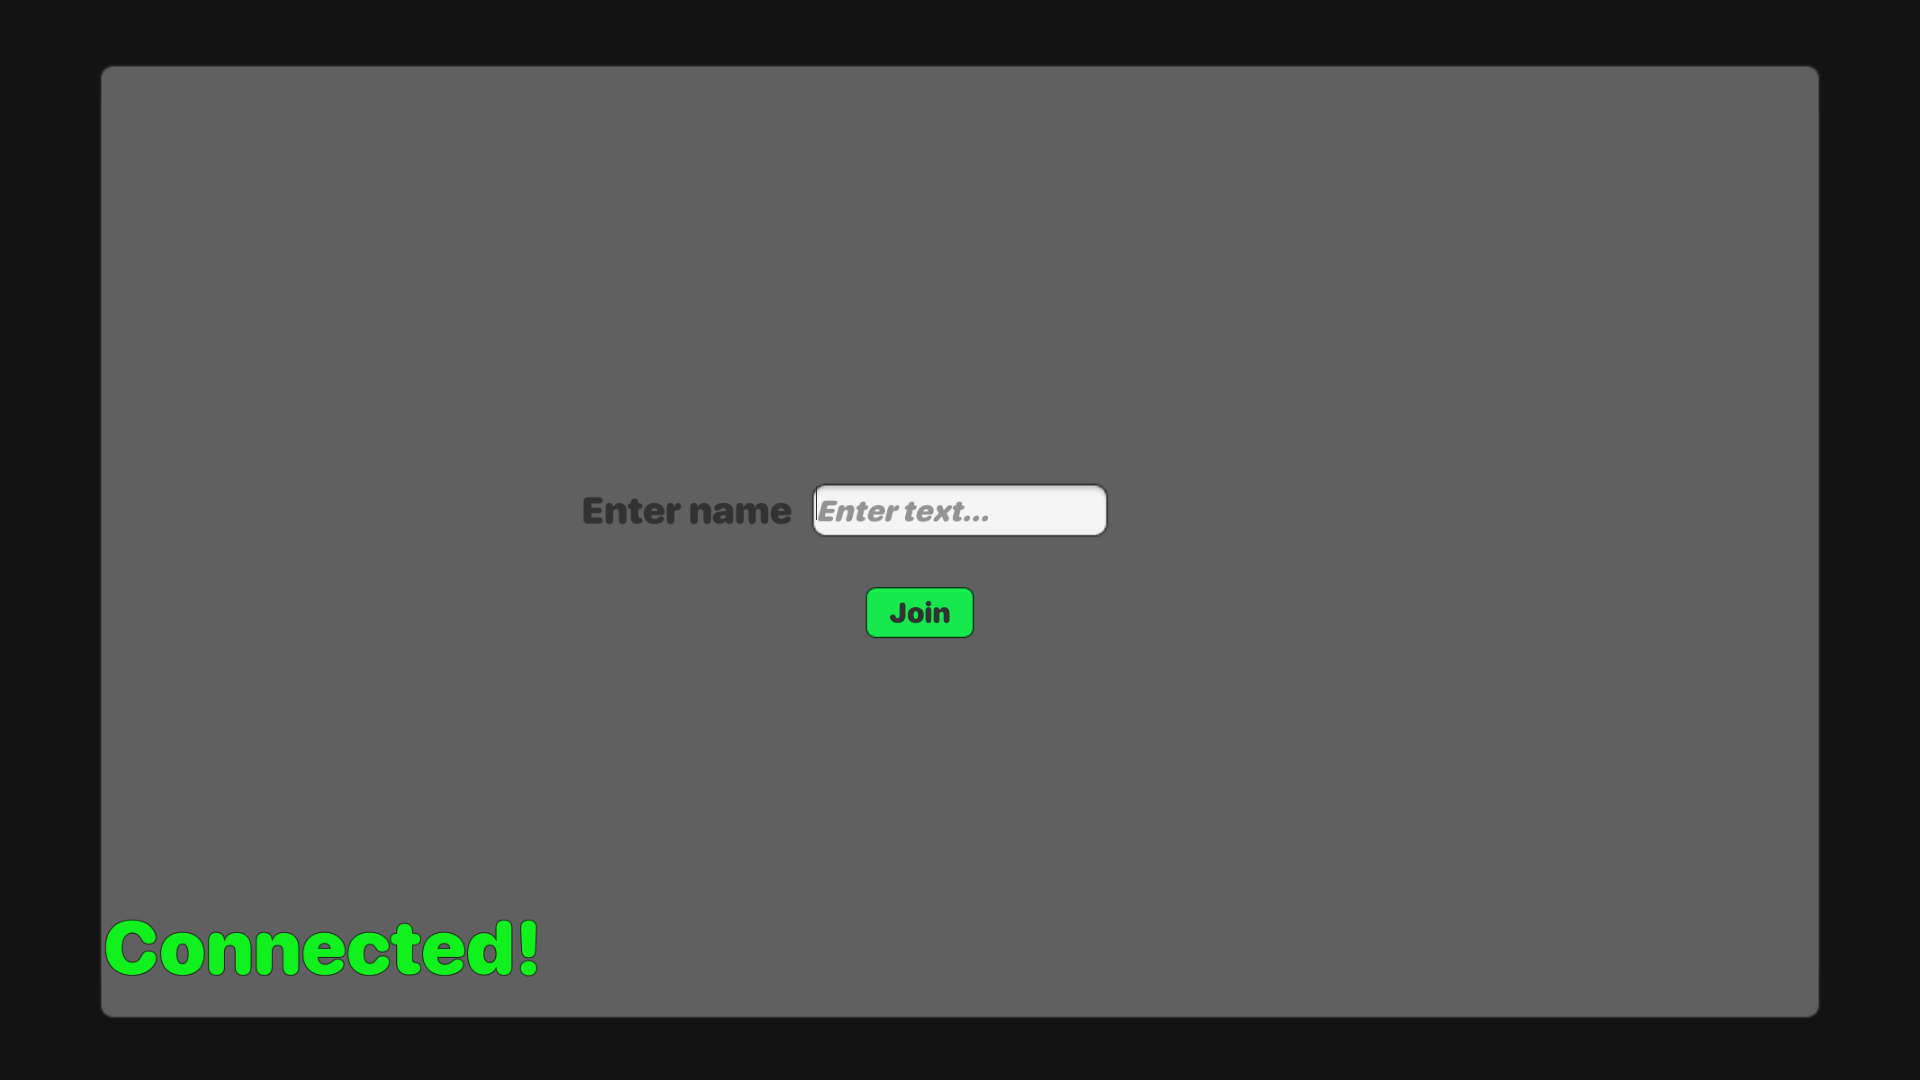
\includegraphics[scale=0.2]{image21.png}
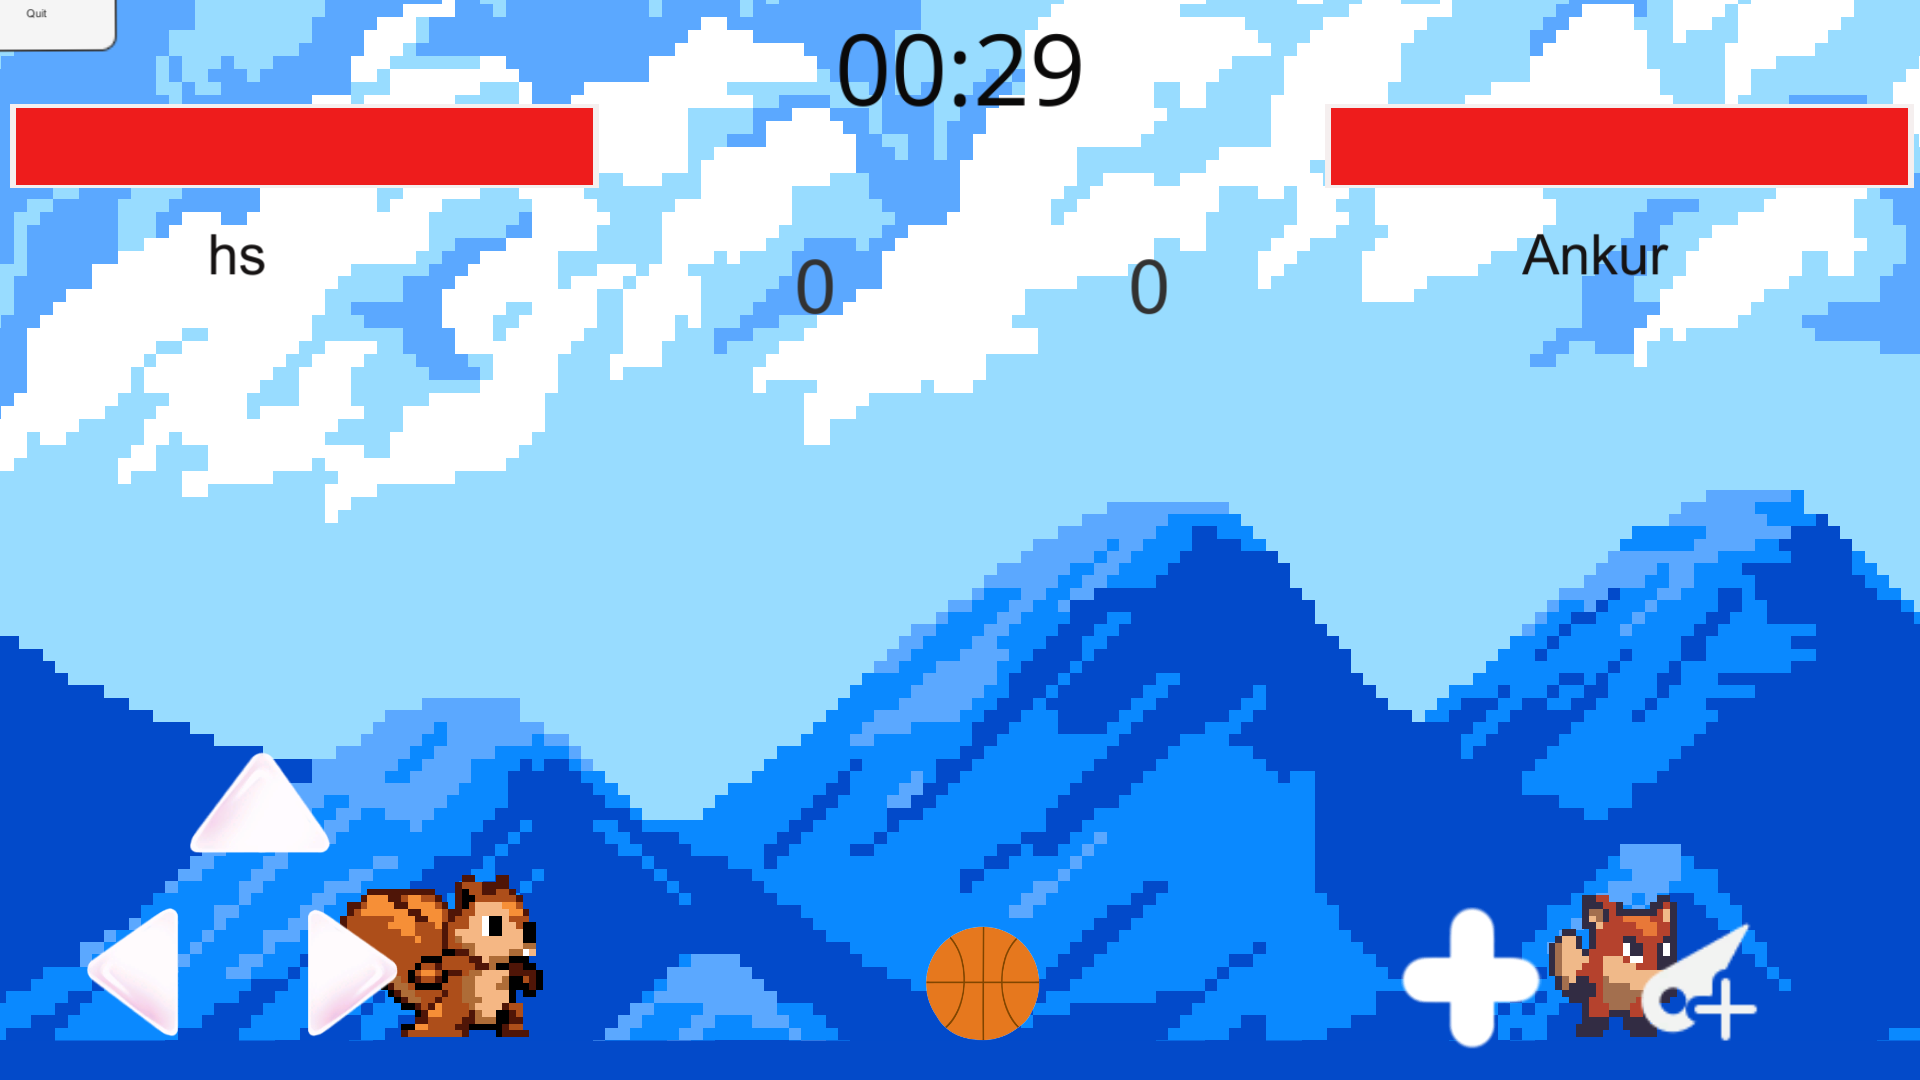
\includegraphics[scale=0.2]{image22.png}
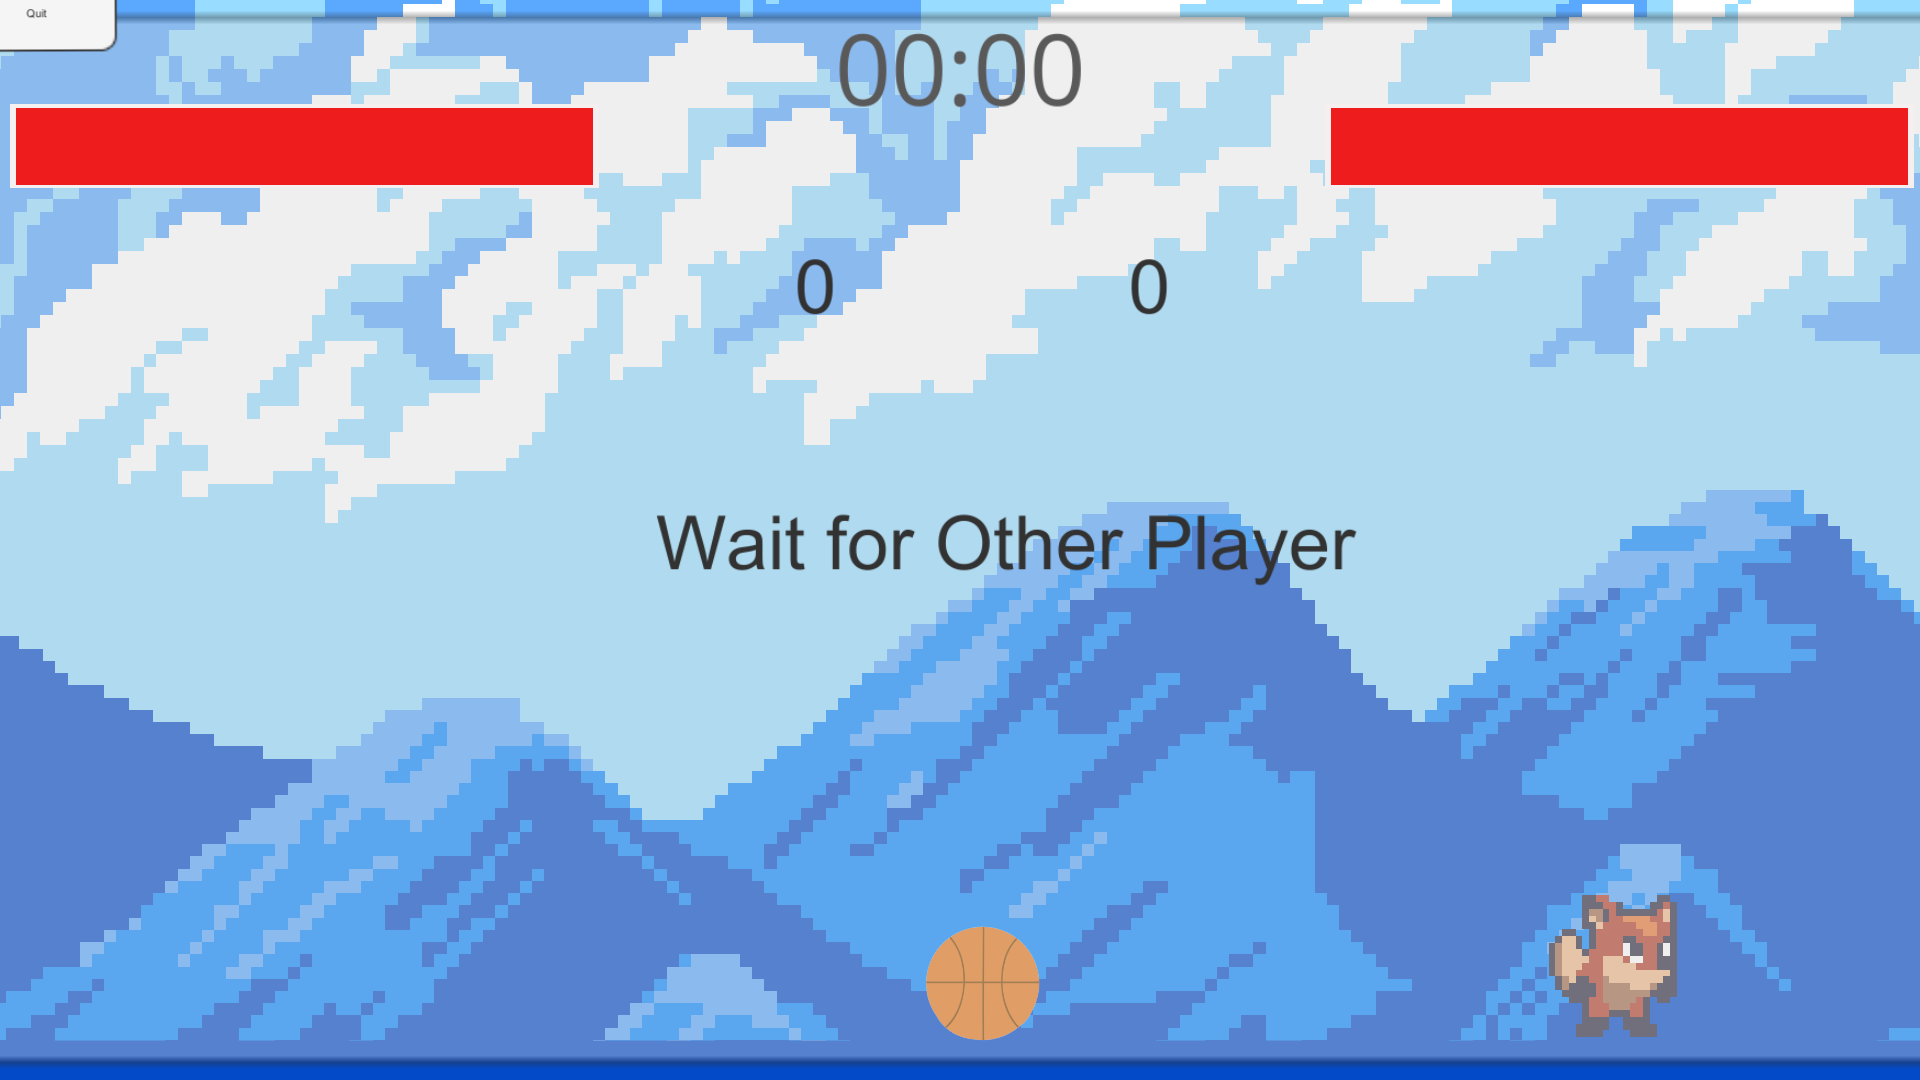
\includegraphics[scale=0.2]{image23.png}
\end{center}
\newpage
\textbf{Future Updates}

\begin{center}
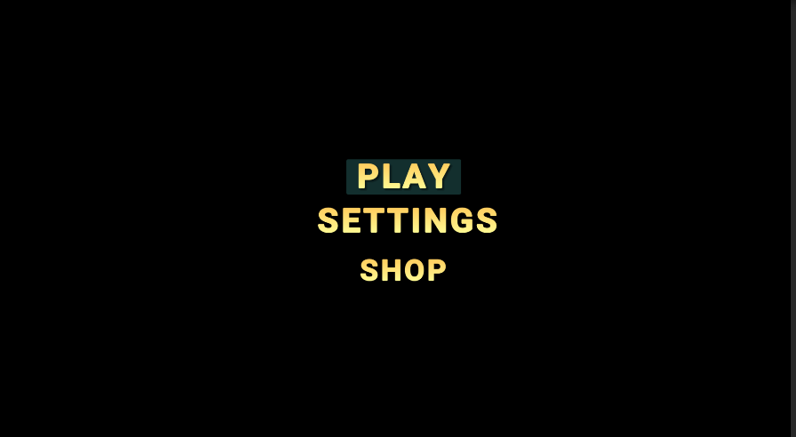
\includegraphics[scale=0.7]{image24.png}

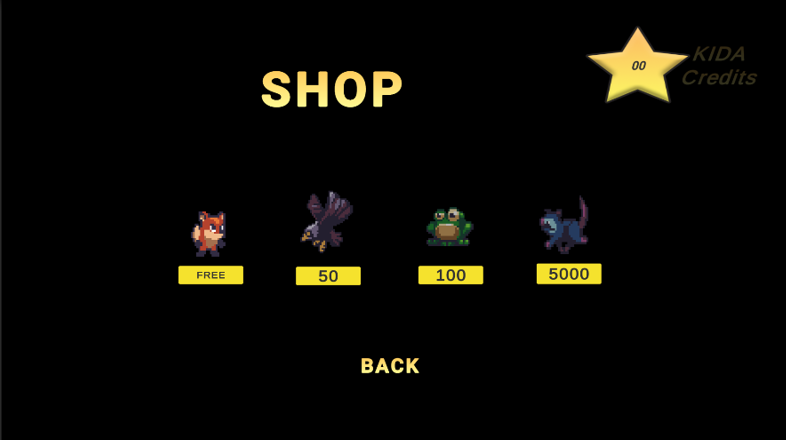
\includegraphics[scale=0.7]{image25.png}
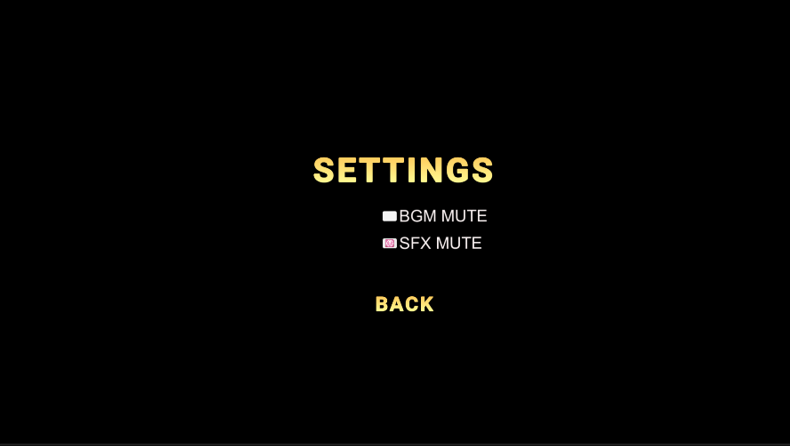
\includegraphics[scale=0.7]{image26.png}
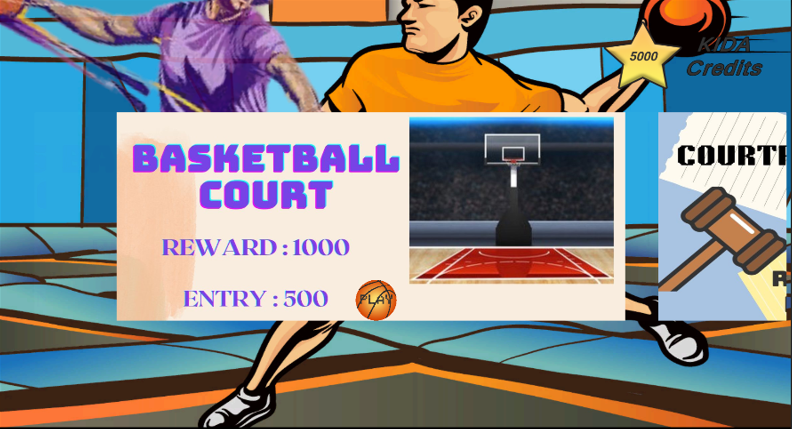
\includegraphics[scale=0.7]{image27.png}
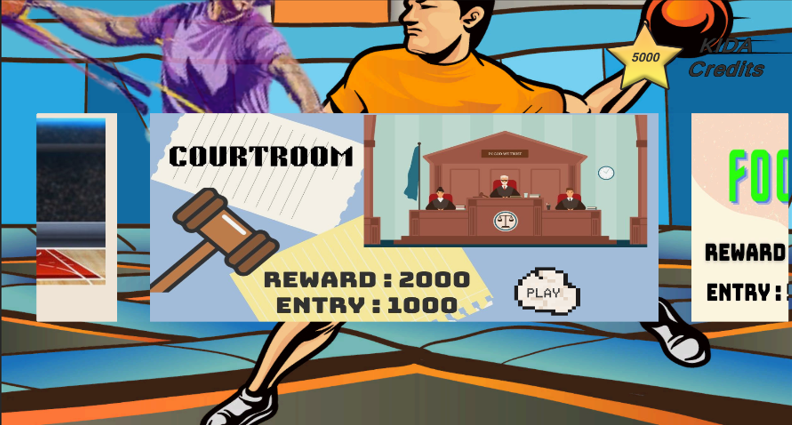
\includegraphics[scale=0.7]{image28.png}
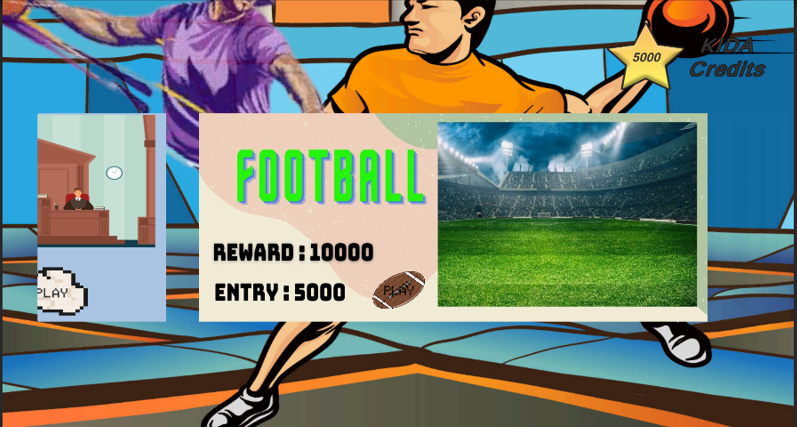
\includegraphics[scale=0.7]{image29.png}
\end{center}



\vspace{1cm}

\clearpage
\centering
\section{TESTING}
\justifying
\setlength{\parindent}{4em}
\setlength{\parskip}{0.5em}
\renewcommand{\baselinestretch}{1.5}
\normalsize
\subsection{INTRODUCTION}
\hspace{1.7 cm}Testing is an important part of software development life cycle. It is performed to ensure 
quality of the developed system. Testing includes a set of investigative activities that can be 
planned in advance and conducted systematically, to assure the stakeholder that system 
fulfils all the requirements gathered during requirement gathering phase. Software testing is 
one of the key elements in software projects that is often referred to as verification and 
validation. Verification refers to the set of activities that ensure that software correctly 
implements specified functionality. Validation refers to a set of activities built around 
traceability matrix which ensure that the functionality implemented by the system is 
traceable to customer requirements

Tests are the individual tests specified in a test plan document. Each test is typically 
described by
\begin{itemize}
\item An initial system state.
\item A set of actions to be performed.
\item The expected results of the test.
\end{itemize}

\subsection{IMPLEMENTATION}
\justifying
\setlength{\parindent}{4em}
\setlength{\parskip}{0.5em}
\renewcommand{\baselinestretch}{1.5}
\normalsize

Test cases are planned in accordance to the test process and documented with detailed test 
descriptions. These test cases use cases based on projected operational mission scenarios. 
The testing process also includes stress or load testing for stability purpose (i.e., at 95% CPU 
use, system stability is still guaranteed. The test process thoroughly tests the interfaces and 
modules. Software testing includes a traceable white box testing, black box testing and other 
test processes verifying implemented software against design documentation and 
requirements specified.


\subsection{OBJECTIVE}
\justifying
\setlength{\parindent}{4em}
\setlength{\parskip}{0.5em}
\renewcommand{\baselinestretch}{1.5}
\normalsize

The software test plan (STP) is designed to test each module to measure its performance, to 
uncover bugs in the system, to set aright any flaws in logic that may be present, and to check 
logical flow from one module to another within system.
\begin{itemize}
\item All field entries must work properly.
\item Pages must be activated from the identified link.
\item The entry screen, messages and responses must not be delayed.

\end {itemize}


\subsection{TESTING STRATEGY}
\justifying
\setlength{\parindent}{4em}
\setlength{\parskip}{0.5em}
\renewcommand{\baselinestretch}{1.5}
\normalsize

A strategy outlines what to plan, and how to plan it. A successful strategy is your guide 
through change, and provides a firm foundation for ongoing improvement. Unlike a plan, 
which is obsolete from the point of creation, a strategy reflects the values of an organization 
- and remains current and useful. When an organization tests its products or its tools, it tries 
to compare them against its expectations and values. By its nature, testing introduces change 
as problems are identified and resolved. A test strategy is necessary to allow these two 
impulses to work together. Furthermore, testing can never be said to be ‘complete’, and a 
core skill in testing is the justified management of conflicting demands; without a strategy, 
these judgements will be inconsistent to the point of failure.\\
Software development is a creative process. A test strategy is a vital enabler to this process 
keeping focus on core values and consistent decision-making to help achieve desired goals 
with best use of resource. 

\subsection{TYPES OF TESTING}
\justifying
\setlength{\parindent}{4em}
\setlength{\parskip}{0.5em}
\renewcommand{\baselinestretch}{1.5}
\normalsize

\hspace{1.7 cm} 
1. Unit Testing:
Test individual components or functions of the game, such as player movement, ball physics, and scoring logic, to ensure they work correctly in isolation.

2. Integration Testing:
Test the interaction between different components of the game, such as how player input affects movement, how the ball interacts with the environment, and how the game state updates based on player actions.

3. System Testing:
Test the entire game as a whole to ensure that all components work together seamlessly and that the game meets its requirements and specifications.

4. Compatibility Testing:
Test the game on different platforms, devices, and operating systems to ensure it works correctly and consistently across various environments.

5. Performance Testing:
Test the game under various loads and conditions to ensure it maintains optimal performance, such as handling multiple players, managing network latency, and maintaining frame rates.

6. Load Testing:
Test the game's ability to handle a large number of simultaneous players to ensure the game server and infrastructure can support the expected player base.

7. Playtesting:
Have real players play the game to gather feedback on game mechanics, balance, and overall enjoyment. This can help identify issues that may not be apparent during other testing phases.

8. Regression Testing:
Test the game after updates, bug fixes, or new features have been implemented to ensure that existing functionality has not been negatively affected.



\subsection{UNIT TESTING}
\justifying
\setlength{\parindent}{4em}
\setlength{\parskip}{0.5em}
\renewcommand{\baselinestretch}{1.5}
\normalsize

Unit testing is used to check the execution path of the module, function, and procedure of 
the system. Test is conducted with the help of normal data and abnormal data. This testing 
includes the different factors like statement coverage, branch coverage, loop processing, 
abnormality, and circulation etc. With the help of this Unit testing we check that all the 
statement in the code is executed or not so it avoids the dead code statement. It checks all 
the branches and execution path of the code. It ensures that all the internal method of 
program are executed and properly integrated with program.

Unit testing involves the design of test cases that validate that the internal program logic is 
functioning properly, and that program inputs produce valid outputs. All decision branches 
and internal code flow should be validated. It is the testing of individual software units of 
the application .it is done after the completion of an individual unit before integration. This 
is a structural testing, that relies on knowledge of its construction and is invasive. Unit tests 
perform basic tests at component level and test a specific business process, application, 
and/or system configuration. Unit tests ensure that each unique path of a business process 
performs accurately to the documented specifications and contains clearly defined inputs 
and expected results.

\subsection{INTEGRATED SYSTEM}
\justifying
\setlength{\parindent}{4em}
\setlength{\parskip}{0.5em}
\renewcommand{\baselinestretch}{1.5}
\normalsize

In integrated testing, all the modules are checked together to ensure that all the modules are 
executing together according to the program specification. Once all the mod ules have been 
tested individually, the most legitimate question can be asked is that when all the modules 
are working properly, why there is need of integrated testing.

The answer is, though all modules are working properly problem may occur while interfacing 
individual module. Testing is event driven and is more concerned with the 
basic outcome of screens or fields. Integration tests demonstrate that although the components 
were individually satisfaction, as shown by successfully unit testing, the combination of 
components is correct and consistent. Integration testing is specifically aimed at exposing the 
problems that arise from the combination of components.

\subsection{FUNCTIONAL TEST}
\justifying
\setlength{\parindent}{4em}
\setlength{\parskip}{0.5em}
\renewcommand{\baselinestretch}{1.5}
\normalsize

Functional tests provide systematic demonstrations that functions tested are available as 
specified by the business and technical requirements, system documentation, and user 
manuals. Functional testing is centered on the following items: Valid Input: identified classes 
of valid input must be accepted. Invalid Input: identified classes of invalid input must be 
rejected. Functions: identified functions must be exercised. Output: identified classes of 
application outputs must be exercised. Systems/Procedures: interfacing systems or procedures 
must be invoked.

Organization and preparation of functional tests is focused on requirements, key functions, or 
special test cases. In addition, systematic coverage pertaining to identify Business process 
flows; data fields, predefined processes, and successive processes must be considered for 
testing. Before functional testing is complete, additional tests are identified and the effective 
value of current tests is determined.




\clearpage


\centering

\section{TEST CASES}

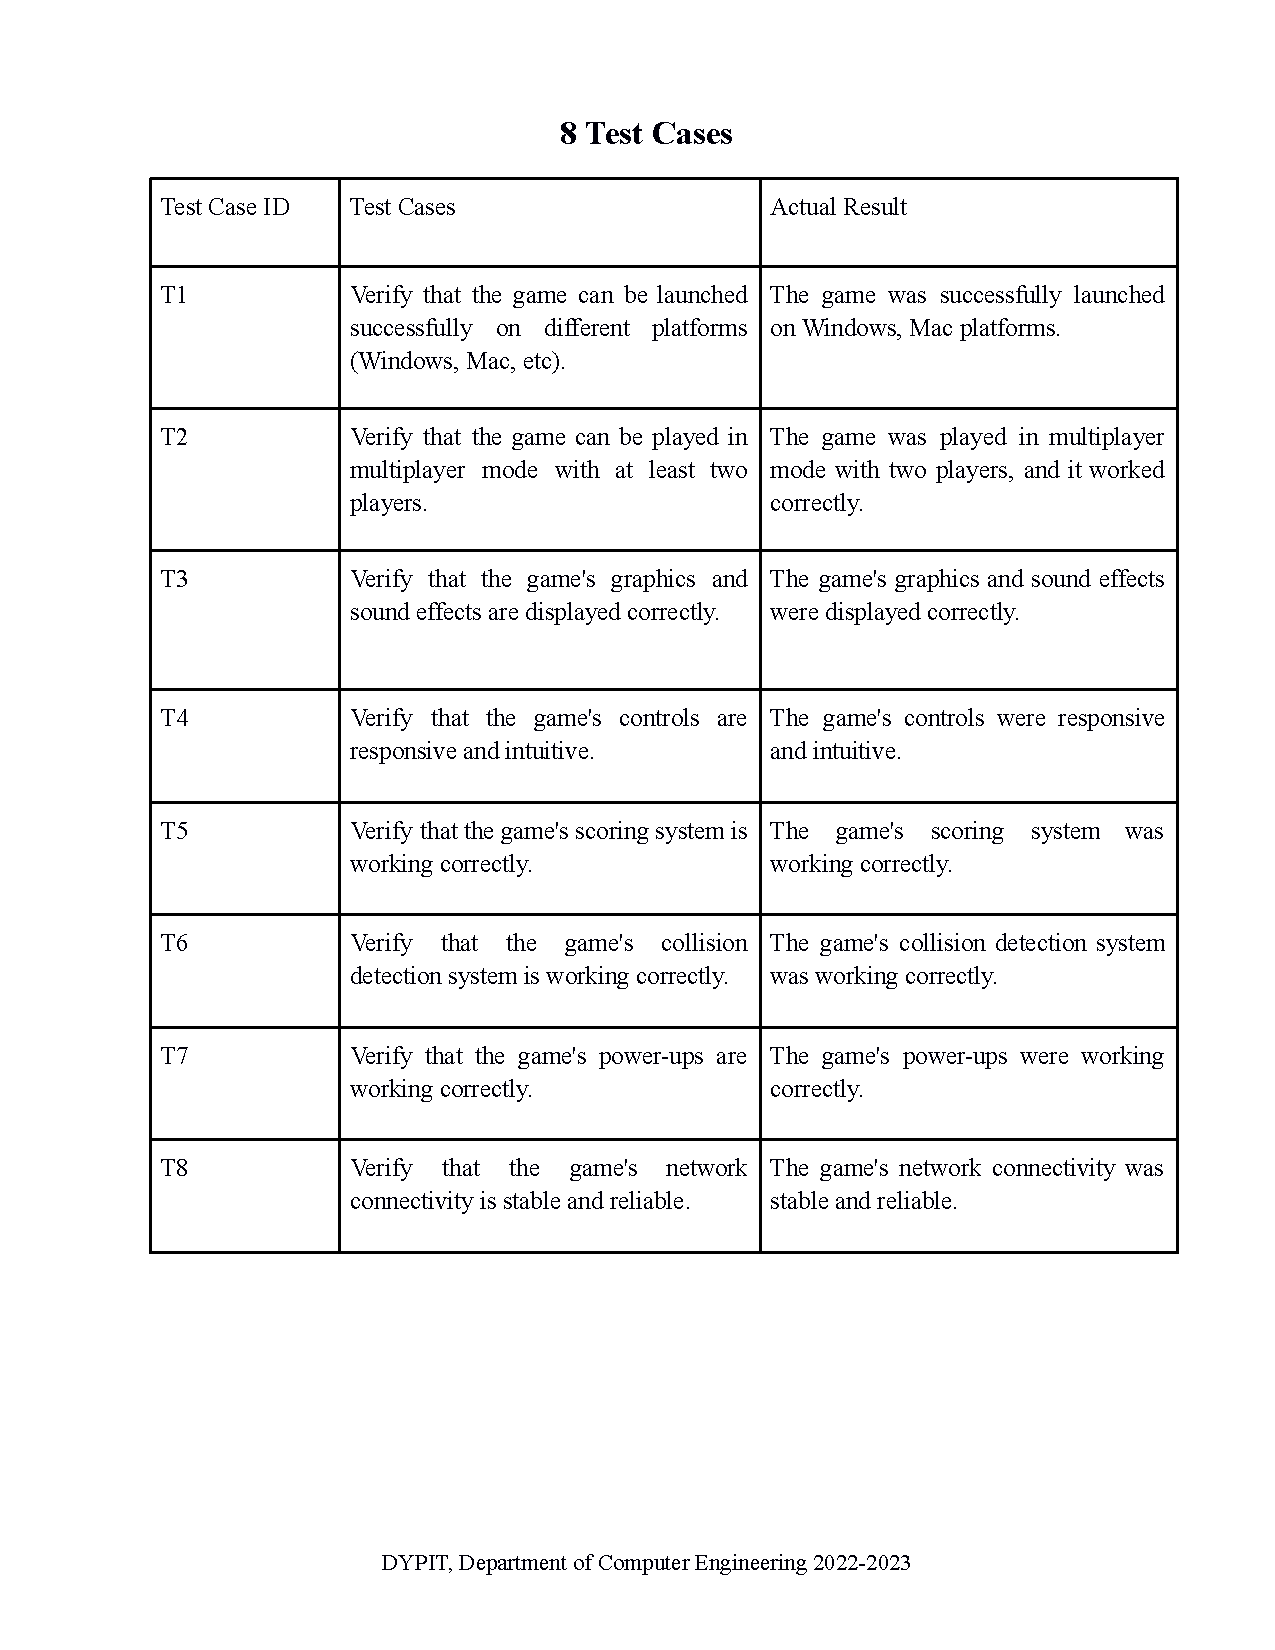
\includepdf[pages={1-} ,offset=0cm 0cm]{TestCase_WithTitle.pdf}
% \includepdf[pages={2-} ,offset=0cm 0cm]{Testing.pdf}


% start conclusion
\centering
\section{CONCLUSION }
\justifying
\setlength{\parindent}{4em}
\setlength{\parskip}{0.5em}
\renewcommand{\baselinestretch}{1.5}
\normalsize

\hspace{1.7cm}
Defining appropriate matchmaking is the first step in developing a matchmaking system.
If you don't offer the machine the rules for what that actually implies,
no algorithm can come up with good matches.
I've talked about our regulations in this post,
which are primarily centered on skill, ping, and pre-made.
You can change how the rules are defined or add new rules depending on what is important for your game. 
\\
\vspace{15cm}

\subsection{APPLICATIONS}
\begin{itemize}
    \item \textbf{Interactive Experience}
        These touchscreen devices are popping up everywhere. Traditional maps in malls have been replaced with interactive touchscreen maps, McDonald's now offers a touchscreen experience for ordering groceries, and major movie theater chains now have kiosks to purchase tickets. All of these solutions require a rich multimedia platform to run them, and the popularity of such solutions is undiminished. Unity's extensibility allows integration with the existing backends these companies already have, and Unity's powerful graphics capabilities make it easy to visually blow people's minds. Again, Unity's various export options allow building on any platform that supports a touchscreen interface.
    \item \textbf{Architectural Visualization}
        Video game engines like Unity can already handle large amounts of complex geometry and render realistic lighting and surfaces. Exploring virtual buildings for engineering and architectural purposes is easy with a game engine like Unity. It's fairly easy to import data from Sketchup or Revit directly into Unity and add Unity's high-end graphics capabilities. Architects can not only look at client concept renders and blueprints, but also use game engines to create 3D experiences that can be delivered to client mobile, desktop, or web browsers. We actually built the Cinema Suite ourselves.
    \item \textbf{Previsualization of Film}
    This one is quite similar to the animation, but not exactly the same. Live action filmmaking requires a lot of advance planning: in many cases, the more planning the better. Drawing traditional scenarios can be a good starting point, but sometimes it can be useful to have a more detailed and realistic approximation of what these scenes will look like. With Unity, Asset Store and The Cinema Suite it is very much possible. As we discussed with Animation, Unity and Cinema Director (part of Cinema Suite) can work together to create great animated sequences in Unity.

    With our Cinema Pro Cams, you can use the same real-world lenses you'd find on set right in the Unity game engine, so you can tell more precisely what your final shot will look like. Cinema Mocap 2 and our soon to be released facial motion capture tool will be great for making your characters move with very little effort. You can find many props, characters, environments and building tools in Unity's Asset Store. It's a great way to populate your virtual scene. Finally, you can use Cinema Director to time and approximate how your movie will look when it's shot and edited.
    
\end{itemize}

% end of appendix
\newpage
\centering
\Large\textbf{ANNEXURE B}

\centering

\Large\textbf{APPENDIX B}\\
\justifying
\setlength{\parindent}{4em}
\setlength{\parskip}{0.5em}
\renewcommand{\baselinestretch}{1.5}
\normalsize
\raggedright\textbf{Details of game deployment:} "itch.io" is an open marketplace for independent digital creators with a focus on independent video games.
\href{https://sharanthakur.itch.io/infinite-pleasure-dodgeball}{Our Games link on Itch.io our deployment platform of choice.}

\vspace{1cm}


\vspace{0.1cm} 






\vspace{15 cm}

\clearpage

\centering

\Large\textbf{APPENDIX C}\\
\justifying
\setlength{\parindent}{4em}
\setlength{\parskip}{0.5em}
\renewcommand{\baselinestretch}{1.5}
\large
\raggedright\textbf{Plagarism Report:}
\vspace{1cm}

\begin{figure}[h]
\centering
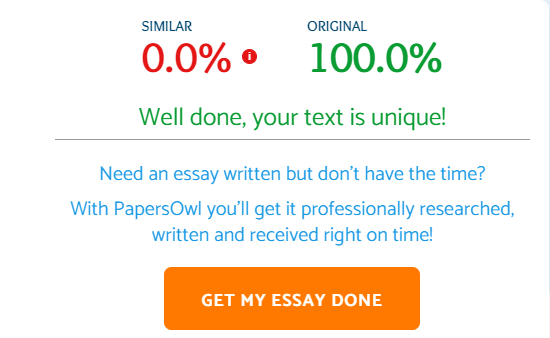
\includegraphics[scale=0.9]{image32.png}

\end{figure}
\vspace{15 cm}


% start of References
\centering
\section{REFERENCES}

\justifying
\setlength{\parindent}{4em}
\setlength{\parskip}{0.5em}
\renewcommand{\baselinestretch}{1.5}
\normalsize

\begin{enumerate}

\item Unity Multiplayer Game development with Photon PUN2 [2020]
\linebreak
\href
{https://www.udemy.com/course/unity-multiplayer-game-development-using-photon-2-2019}
{https://www.udemy.com/course/unity-multiplayer-game-development-using-photon-2-2019}

\item Make a 2D Platformer Character with State Machines in Unity
\linebreak
\href
{https://www.udemy.com/course/make-a-2d-platformer-character-in-unity/}
{https://www.udemy.com/course/make-a-2d-platformer-character-in-unity/}

\item Unity 2020 URP Make a juicy 2d Shooter prototype
\linebreak
\href
{https://www.udemy.com/course/unity-2020-urp-how-to-make-a-2d-roguelike-shooter/}
{https://www.udemy.com/course/unity-2020-urp-how-to-make-a-2d-roguelike-shooter/}

\item Research on the 3D Game Scene Optimization of Mobile Phone Based on the Unity 3D Engine | IEEE Conference Publication
\linebreak
\href
{https://ieeexplore.ieee.org/document/6086340}
{https://ieeexplore.ieee.org/document/6086340}

\item Developing a game application to encourage face-to-face local gaming experience | IEEE Conference Publication | IEEE Xplore
\linebreak
\href
    {https://ieeexplore.ieee.org/document/8052656}
    {https://ieeexplore.ieee.org/document/8052656}

\item Developing MOBA games using the Unity game engine | IEEE Conference Publication | IEEE Xplore
\linebreak
\href
{https://ieeexplore.ieee.org/document/8052656}
{https://ieeexplore.ieee.org/document/8052656}

\item SOUL: Simulation of Objects in Unity for Learning | IEEE Conference Publication
\linebreak
\href
{https://ieeexplore.ieee.org/document/8968786}
{https://ieeexplore.ieee.org/document/8968786}

\item Computing Games: Bridging the Gap Between Search and Entertainment | IEEE Journals \& Magazine
\linebreak
\href
{https://ieeexplore.ieee.org/document/9427480}
{https://ieeexplore.ieee.org/document/9427480}

\item Game or Watch: The Effect of Interactivity on Arousal and Engagement in Video Game Media | IEEE Journals \& Magazine | IEEE Xplore
\linebreak
\href
{https://ieeexplore.ieee.org/document/9403941}
{https://ieeexplore.ieee.org/document/9403941}


\end{enumerate}
%\subsubsection{WEB RESOURCES}
%\begin{enumerate}
%\item  \href{URL}{www.wikipedia.org}
%\item  \href{URL}{www.sciencedirect.com}
%\item  \href{URL}{www.slideshare.net}
%\end{enumerate}
\clearpage
%end of references


% seminar report documentation


\end{document}
